This Section contains an overview of the methodology used for a time-dependent measurement of the Z boson production at ATLAS. The methodology follows that presented in the Z-counting luminosity measurement~\cite{ATL-DAPR-PUB-2021-001}, with the software framework used having been transferred to AnalysisBase, opposed to the online monitoring framework initially used in Z-counting.

The methodology was first established as an alternative measurement of the luminosity recorded by the ATLAS experiment, where the Z-boson decay into dileptons during physics running is used to provide additional checks against residual time, pile-up or beam-condition-dependent biases that may affect the baseline ATLAS luminosity values, which determination is detailed in Ref~\cite{ATLAS-CONF-2019-021}.

The Drell-Yan production of dilepton pairs is a well understood process, with the clean Z-boson signature of two high-transverse momentum, oppositely charged leptons\footnote{Z-boson decays to $\tau$ leptons or quarks are not considered here, as they are much more difficult to reconstruct and prone to very high background levels.} providing robustness against varying pileup conditions. Thus, a luminosity measurement can be obtained by measuring the number of produced Z-bosons, $N_Z$, using the formula

\begin{equation}
\mathcal{L}_Z = \frac{N_Z}{\sigma_Z}
\label{eq:Zcount:RawLumi_app}
\end{equation}

where $\sigma_Z$ is the Z production cross section. Experimentally, precise measurements of $\sigma_{Z\rightarrow e^+e^-}$ ($\sigma_{Z\rightarrow \mu^+\mu^-}$) have been obtained with systematic uncertainties (excluding luminosity) of about 1.0\% (1.5\%)~\cite{ATLAS:2019zci}. The value of the $Z\rightarrow \ell^+\ell^-$ cross-section is predicted by calculations at next-to-next-to-leading order QCD with a total uncertainty of 3-4\% at 90\% CL, where the uncertainty is driven by the current knowledge of the proton parton distribution functions (PDFs). As the uncertainties in the baseline ATLAS luminosity are below 2\%~\cite{ATLAS-CONF-2019-021}, the Z-counting luminosity is not competitive as an absolute measurement, but has many powerful features as a relative luminometer.

The Z-counting procedure is performed as a function of time, in units of "luminosity blocks" (LBs), the smallest time interval for which luminosities are measured in ATLAS. These typically correspond to 60 seconds intervals, but occasionally account for a shorter amount of time depending on trigger or data acquisition configurations.

\subsection{Data samples and event selection}
\label{sec:Zcount:Event selection}

The analysis presents the results for the full high-luminosity ATLAS Run 2 dataset, recorded between 2015 and 2018 for $pp$ collisions at $\sqrt{s}=13$~TeV, amounting to a total integrated luminosity of approximately 139~$fb^{-1}$. The dataset is divided within ATLAS into 595 runs, where one run typically corresponds to one LHC fill.

Events passing unprescaled single-lepton triggers with a transverse energy (momentum) threshold of 24~GeV (20~GeV) for electron (muon) candidates for 2015 data and of 26~GeV for 2016-18 data, within the pseudorapidity range of $|\eta|<2.4$. Events with at least two well-identified and isolated leptons with the same flavour and opposite charge are selected, where either (or both) of the leptons pass the single-lepton trigger requirements aforementioned. A likelihood based identification criterion is applied to the electron candidates, using the LHMedium working point~\cite{ATLAS:2019jvq}. The muon candidates are required to be reconstructed from a combination of inner detector (ID) and muon spectrometer (MS) tracks and pass Medium identification criteria~\cite{ATLAS:2016lqx}. Both electrons and muons are required to satisfy the Loose\_VarRad isolation criteria.

Electron and muon candidates are required to originate from the primary vertex of the event, defined as the vertex with at least two reconstructed racks with a transverse momentum greater than 0.4~GeV and the highest sum of squared transverse momenta of associated tracks. This is achieved by requiring the significance of the candidate track's transverse impact parameter, calculated relative to the beam line, $|d_0|/\sigma_{d_0}$ to be smaller than 3.0 for muon candidates and 5.0 for electron candidates. Additionally, the longitudinal impact parameter $z_0$, defined as the difference between the $z$-coordinate of the point of closest approach to the beam line and the longitudinal position of the primary vertex, is required to satisfy $|z_0\sin\theta|<0.5$~mm.

The selection requirements are listed in Table~\ref{tab:Zcount:LeptonSele}, where the phase-space boundaries are determined by the transverse momentum ($p_\text{T}$) and pseudorapidity ($\eta$) ranges. All leptons passing these requirements will be referred to as "good" leptons, with a same-flavour, oppositely-charged pair of these is required to form a $Z$ boson candidate, with an additional requirement on their invariant mass of $66<m_{\ell\ell}<116$~GeV.

\begin{table}[!htb]
	\centering
	\begin{tabular}{@{}ccc@{}}
		\toprule
		\textbf{Selection criteria}               & \textbf{Electron channel}	& \textbf{Muon channel}	 \\ \midrule
		Transverse momentum                       & $p_\text{T}^e>27$~GeV	& $p_\text{T}^\mu>27$~GeV 	\\
		Pseudorapidity                            & $0<|\eta^e|<1.37$ or $1.52<|\eta^e|<2.4$	& $0.<|\eta^\mu|<2.4$	\\
		Identification                            & LHMedium	& Medium, ID+MS combined muon	\\
		Isolation                                 & Loose\_VarRad & Loose\_VarRad \\
		\multirow{2}{*}{Track-vertex association} & $|z_0\sin\theta|<0.5$~mm & $|z_0\sin\theta|<0.5$~mm \\
		& $|d_0|/\sigma(d_0)<5$	& $|d_0|/\sigma(d_0)<3$                                      \\
		Invariant mass                            & $66<m_{e^+e^-}<116$~GeV & $66<m_{\mu^+\mu^-}<116$~GeV \\ \bottomrule
	\end{tabular}
	\caption{Overview of selection criteria, where each criterion is applied to a single lepton and two oppositely charged leptons of the same flavour are required to form a Z-boson candidate, with invariant mass in the range 66 to 116$\sim$GeV. The fiducial phase space is flavour-specific, and determined by the invariant-mass, $|\eta^\ell|$ and $p_\text{T}^\ell$ requirements.}
	\label{tab:Zcount:LeptonSele}
\end{table}

\subsection{Luminosity determination}

For each lepton flavour the raw rate of detected $Z$s is measured on a LB-by-LB basis. To obtain the $Z$ production rate, the raw rate is corrected to account for the trigger and reconstruction efficiencies. These data-driven efficiencies are subject to additional corrections, derived as a function of the average number of simultaneous collisions, $\left< \mu \right>$, from Monte Carlo simulations. A small background subtraction is also applied in order to account for dilepton pairs in the event selection phase space originating from diboson and $t\bar{t}$ events.

Thus, the general form for calculating the $Z$-counting based instantaneous luminosity as shown in Eq~\ref{eq:Zcount:RawLumi_app} has to be modified as follows

\begin{equation}
\mathcal{L}_{Z\rightarrow \ell^+\ell^-} (LB) = \frac{N_{Z\rightarrow \ell^+\ell^-}(LB)\cdot (1-f_\text{bkg})}{\sigma_\text{theo}\times A^\text{MC}_{Z\rightarrow \ell^+\ell^-}\cdot \varepsilon^\text{T\&P}_{Z\rightarrow \ell^+\ell^-}(LB) \cdot F^\text{MC}_{Z\rightarrow \ell^+\ell^-}(\left< \mu \right>)\cdot t(LB)}
\label{eq:Zcount:ZLumi_app}
\end{equation}

where

\begin{itemize}
	\item $N_{Z\rightarrow \ell^+\ell^-}(LB)$ is the number of selected $Z$ candidates per LB, as defined in the previous section.
	\item $f_\text{bkg}$ is the fraction of background events in the signal region. The value is taken as $f_\text{bkg}=0.005$ in both the electron and muon channels, determined from Monte Carlo studies~\cite{ATLAS:2019zci}.
	\item $\sigma_\text{theo}$ is the inclusive $Z\rightarrow \ell^+\ell^-$ cross-section determined for the range $m_{\ell\ell}>60$~GeV to select the inclusive invariant mass range of the simulated $Z$ events. The value used is $\sigma_\text{theo}=1970$~pb, with a PDF uncertainty of 3.5\% at 90\% CL, obtained at NNLO QCD theory with the FEWZ 3.1.b2 framework~\cite{PhysRevD.86.094034} using the CT18ANNLO proton PDF~\cite{Hou:2019efy}. All results in the analysis will either base on $\mathcal{L}_{Z\rightarrow e^+e^-}/\mathcal{L}_{Z\rightarrow \mu^+\mu^-}$ ratios, or normalised to the integrated baseline ATLAS luminosity values, cancelling the dependence on this value and its uncertainty.
	\item $A^\text{MC}_{Z\rightarrow \ell^+\ell^-}$ is an acceptance factor correcting the inclusive cross-section $\sigma_\text{theo}$ to the fiducial phase space defined in Table~\ref{tab:Zcount:LeptonSele}.
	\item $\varepsilon^\text{T\&P}_{Z\rightarrow \ell^+\ell^-}(LB)$ is the event trigger and reconstruction efficiency obtained per LB from the data-driven tag-and-probe procedure discussed in Section~\ref{sec:Zcount:Data driven effs}.
	\item $F^\text{MC}_{Z\rightarrow \ell^+\ell^-}(\left< \mu \right>)$ is a correction factor for efficiency effects beyond the ones determined in the tag-and-probe procedure, derived from Monte Carlo as a function of the average pileup, $\left< \mu \right>$. Further details found in Section~\ref{sec:Zcount:MC correction factor}.
	\item $t(LB)$ is the live time of typically about 60 seconds per LB. The live time is corrected for detector dead time effects.
\end{itemize}

\subsection{Data-driven efficiency estimation}
\label{sec:Zcount:Data driven effs}

An important aspect of the $Z$-counting method is that electron and muon reconstruction and trigger efficiencies can be calculated using the $Z$ events themselves, correcting for time-dependent detector inefficiencies affecting the boson's detection rate. The efficiency to select a $Z$ event is factorised into single-lepton trigger and reconstruction efficiencies, which are measured independently for each lepton flavour. The combination of these terms results in the $Z$ event-level selection efficiency as a function of time (in units of LBs). This Section outlines the steps of the determination, with figures given for an example run.

\subsubsection{Single-lepton trigger efficiency}

The single-lepton trigger efficiency is defined with respect to the "good" lepton criteria and determined using events with two "good" leptons passing the selection detailed in Table~\ref{tab:Zcount:LeptonSele}. Since the procedure is the same for both lepton flavours the term lepton will be used.

The single-lepton trigger efficiency, $\varepsilon_{\text{trig,}1\ell}$ can be derived by counting the number of events where exactly 1 lepton passed the trigger requirement ($N_1$) and the number of events where both leptons passed the trigger ($N_2$) as follows:

\begin{equation}
	\varepsilon_{\text{trig,}1\ell}=\frac{1}{\frac{N_1}{2N_2}+1}
		\label{eq:Zcount:Single-lep trig eff}
\end{equation}

The statistical uncertainty on this efficiency is calculated by propagating the Poisson counting uncertainties on $N_1$ and $N_2$. Due to the requirements of two isolated and well identified leptons with a dilepton mass close to the $Z$-boson mass range, the background contribution is small and neglected. This formalism assumes that the trigger efficiencies of the two leptons are independent, and therefore neglects the correlation between the two.

The event-level trigger efficency is determined from the single-lepton trigger efficiencies as

\begin{equation}
	\varepsilon_\text{trig,event}=\left( 1 - (1-\varepsilon_{\text{trig,}1\ell})^2 \right)
\end{equation}

\subsubsection{Single-lepton reconstruction efficiency}

For both electrons and muons, the single-lepton reconstruction efficiency is calculated in a tag-and-probe procedure (T\&P) similar to that routinely done for ATLAS physics analyses~\cite{ATLAS:2016lqx, ATLAS:2019qmc}. A high-quality "tag lepton" is selected along with a loose "probe lepton" candidate with the extra requirement that the invariant mass of the tag-and-probe pair be very close to the $Z$-bosom mass. In this note, the reconstruction efficiency is defined as the efficiency of the "good" lepton selection with respect to the loose object, and is determined from the fraction of probes that pass the "good" lepton selection. The efficiency $\varepsilon_{\text{reco},1\ell}$ is not the full efficiency to select a "good" lepton. Specifically, it does not include the efficiency to reconstruct the loose "probe" leptons. Any missing components are estimated entirely from simulation and form part of the correction factors discussed in Section~\ref{sec:Zcount:MC correction factor}.

The tag lepton is required to pass the single-lepton trigger to avoid a trigger bias, and is also required to pass tight selection criteria to ensure it has a low probability of being a mis-identified lepton. As the probe object has much looser selection criteria, mis-identified leptons and combinatorial backgrounds can be significant, so unlike for the trigger efficiency determination the background needs to be taken into account. The single-lepton reconstruction efficiency (indicated with the subscript "reco,1$\ell$") is calculated according to:

\begin{equation}
	\varepsilon_{\text{reco},1\ell}=\frac{N^\text{OS}_\text{pass}-N^\text{bkg}_\text{pass}}{N^\text{OS}_\text{pass}+N^\text{OS}_\text{fail}-N^\text{bkg}_\text{total}}
	\label{eq:Zcount:Single-lep reco eff}
\end{equation}

where $N^\text{OS}_\text{pass}$ ($N^\text{OS}_\text{fail}$) is the number of opposite-charge tag-and-probe pairs where the probe satisfies (fails) the "good" lepton selection criteria and $N^\text{bkg}_\text{total}$ ($N^\text{bkg}_\text{pass}$) are estimates for the background in the denominator (numerator). The statistical uncertainty on this efficiency is calculated using error propagation on all terms in Equation~\ref{eq:Zcount:Single-lep reco eff}.

The selection criteria used to select "tag" and "probe" leptons are listed in Table and are discussed further below. The reconstruction efficiency is calculated only for leptons within the fiducial phase space defined in the preselection criteria listed in Table, while the "probe" selection criteria determine whether a lepton passes or fails.

\begin{table}[!htb]
	\centering
	\begin{tabular}{@{}cccc@{}}
		\toprule
		\textbf{Lepton candidate}           & \textbf{Selection criteria}  & \textbf{Electron channel} & \textbf{Muon channel}                                             \\ \midrule
		\multirow{2}{*}{{\textbf{Tag}}} & Lepton identification        & LHTight                   & As in Table~\ref{tab:Zcount:LeptonSele} \\
		& Single lepton trigger object & Matched                   & Matched                                                           \\ \midrule
		\multirow{7}{*}{\textbf{Probe}}     & \multicolumn{3}{c}{\textbf{Preselection criteria}}                                                                           \\
		& Object                       & Cluster loosely matched to ID track		& ID track\\
		& Transverse momentum          & $p_\text{T}^e>27$~GeV                  	& $p_\text{T}^\mu>27$~GeV \\
		& Pseudorapidity               & $0<|\eta^e|<1.37$ or $1.52<|\eta^e|<2.4$	& $0.<|\eta^\mu|<2.4$ \\
		& Track-vertex association     & -                          &  $|z_0\sin\theta|<2$~mm                                                                 \\
		& \multicolumn{3}{c}{\textbf{Probe selection criteria}}                                                                        \\
		& Requirement                  & Passes all cuts in Table~\ref{tab:Zcount:LeptonSele}  & \begin{tabular}[x]{@{}c@{}}Match to combined muon\\ passing cuts in Table~\ref{tab:Zcount:LeptonSele},\\ with looser $p_\text{T}^\mu>21.6$~GeV cut.\end{tabular} \\ \bottomrule
	\end{tabular}
	\caption{Lepton selection criteria for "tag" and "probe" candidates. Tag candidates are also required to pass all cuts in Table~\ref{tab:Zcount:LeptonSele}. Requirements for the probe selecion criteria determine whether a lepton passes or fail the reconstruction.}
	\label{tab:Zcount:RecoEffSelection}
\end{table}

\paragraph{Electron channel reconstruction efficiency} In the electron channel, the tag electron is required to pass tight identification criteria~\cite{ATLAS:2019jvq} and be matched to a single-electron trigger object, as shown in Table~\ref{tab:Zcount:RecoEffSelection}. The probes are clusters of energy in the electromagnetic calorimeter loosely matched to an ID track with further kinematic requirements, also detailed in Table~\ref{tab:Zcount:RecoEffSelection}. The efficiency for the probe-level selection with respect to true electrons is about 98\% and is well described by the simulation~\cite{ATLAS:2019jvq}. The probability to measure the electron charge correctly is about 99\% and is well described by the simulation.

The nominal selection for the tag-and-probe pairs to be used in Equation~\ref{eq:Zcount:Single-lep reco eff} are opposite-charge pairs with an invariant mass of $75<m_{ee}<105$~GeV, called the peak region, where the probe is either passing or failing the "good" electron selection criteria. The background is estimated using a "template" method, where a background-enriched sample with minimal signal contribution is selected from data by inverting the identification and isolation requirements. The template is normalisedto the high-mass sideband withing the range of $120<m_{ee}<250$~GeV and the background yields are obtained integrating the template over the peak region. In the denominator, the normalisation uses probes failing the "good" electron selection, while in the numerator same-charge pairs are used to ensure a small signal contamination, resulting in a modified expression for $\varepsilon_{\text{reco},1\ell}$ as follows, 

\begin{equation}
	\varepsilon_{\text{reco},1\ell}=\frac{N^\text{OS}_\text{pass,peak}-N^\text{OS}_\text{template,peak}\cdot\frac{N^\text{SS}_\text{pass,tail}}{N^\text{SS}_\text{template,tail}}}{N^\text{OS}_\text{pass,peak}+N^\text{OS}_\text{fail,peak}-N^\text{OS}_\text{template,peak}\cdot\frac{N^\text{SS}_\text{pass,tail}}{N^\text{SS}_\text{template,tail}}}
\end{equation}

The selection and background estimation are illustrated in Figure~\ref{fig:Zcount:Ele tag-and-probe} for and example LHC run.

\paragraph{Muon channel reconstruction efficiency} All muon candidates that pass the "good" selection criteria and are matched to a single muon trigger object are considered as tags, as shown in Table~\ref{tab:Zcount:RecoEffSelection}. In the muon channel, inner detector tracks passing the preselection cuts listed in Table~\ref{tab:Zcount:RecoEffSelection} are used as probes. The efficiency for the probe-level selection with respect to true muons is stable and slightly above 99\%, well described by simulation~\cite{ATLAS:2016lqx}. A pass or fail of the probe is determined by matching the ID track to a combined muon passing the "good" criteria with the $p_\text{T}$ requirement loosened to 21.6~GeV, ensuring that ID tracks at the boundary of $p_\text{T}=27$~GeV can be successfully matched to a combined muon of slightly lower transverse momentum. All tag-and-probe pairs used in Equation~\ref{eq:Zcount:Single-lep reco eff} with the probe passing or failing the "good" muon selection are opposite-charge pairs within a tight invariant mass window of $86<m_{\mu\mu}<96$~GeV to reduce background contamination. Following Ref.~\cite{ATLAS:2016lqx}, the background terms are estimated using a same-charge selection. The selection and background estimation are illustrated in Figure for the same example LHC run as for the electron channel.

\begin{figure}[!htb]
	\centering
	\subfloat{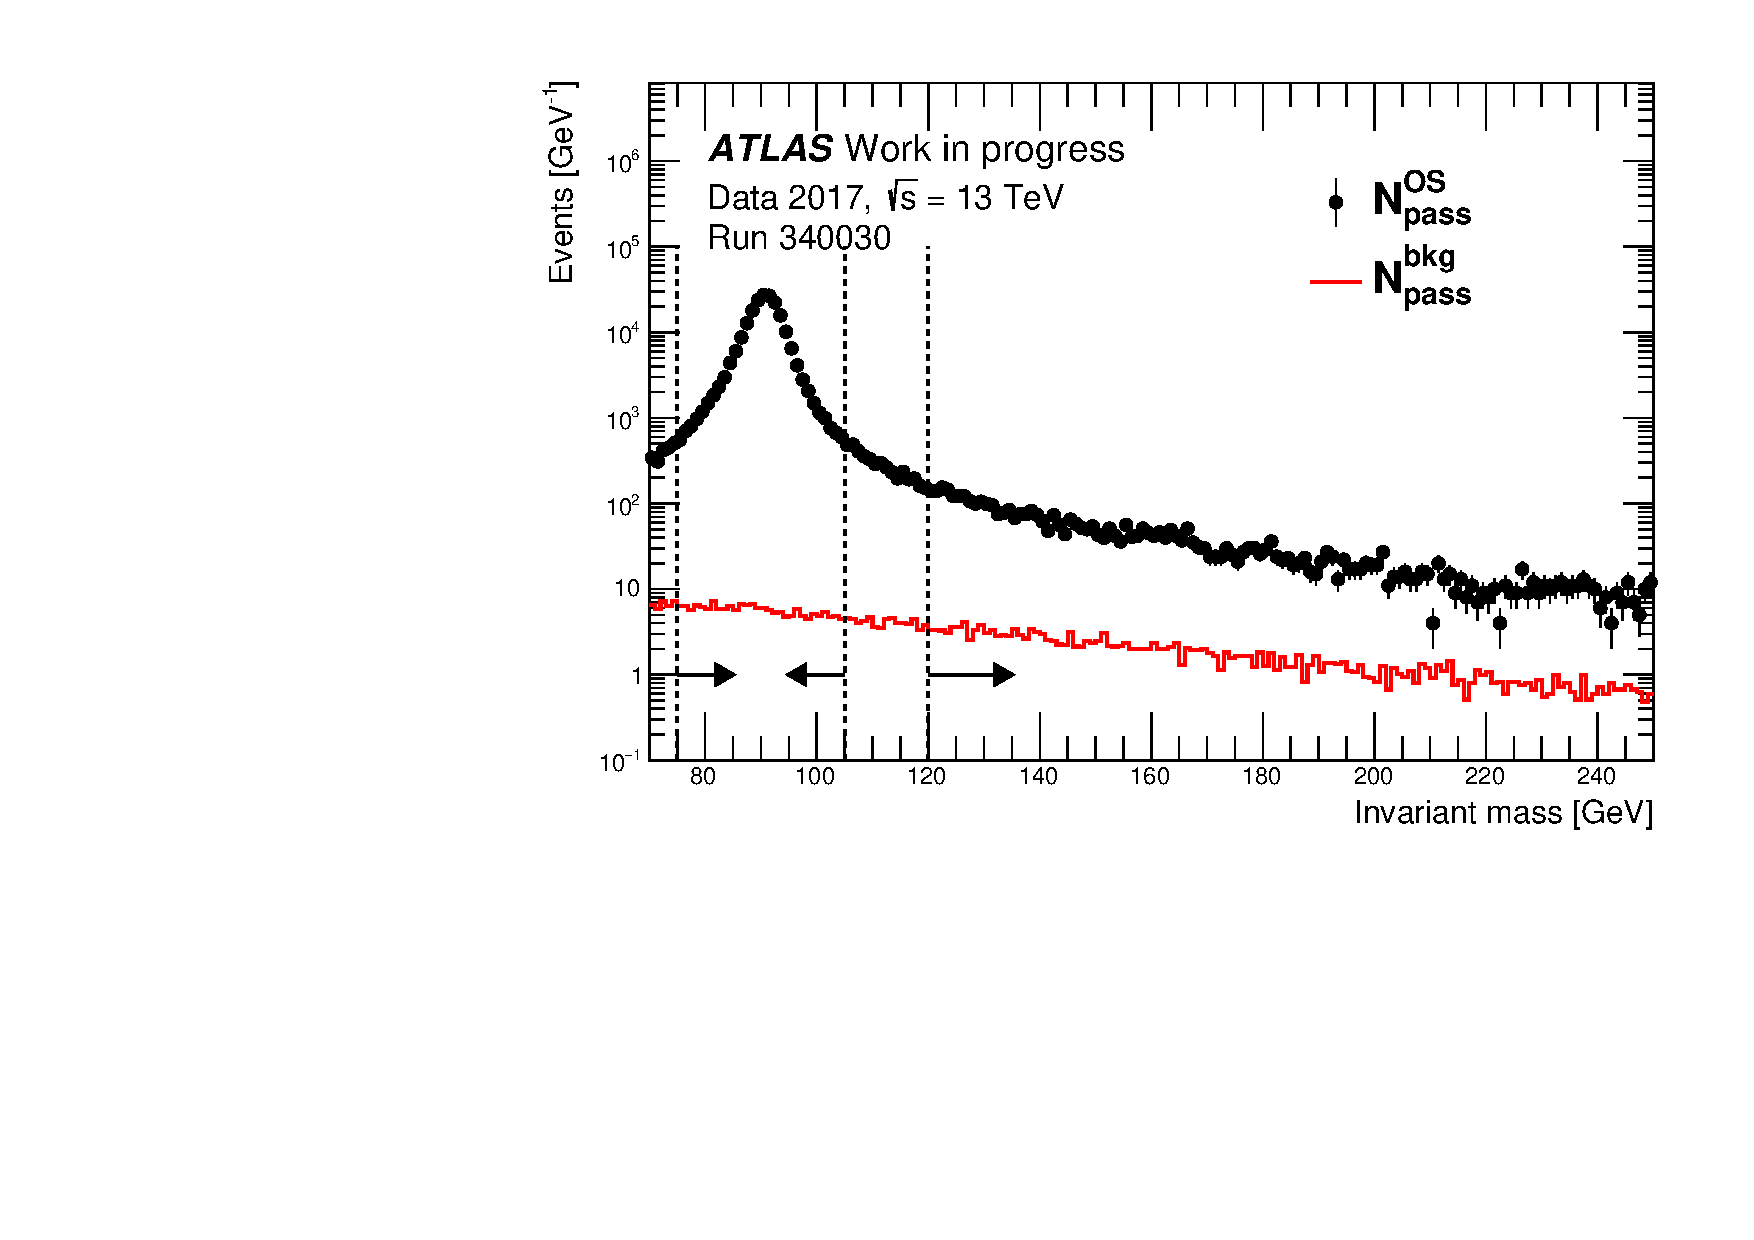
\includegraphics[width=0.48\textwidth]{figs/Zcount/TaP_Numerator_340030_ele.pdf}}
	\subfloat{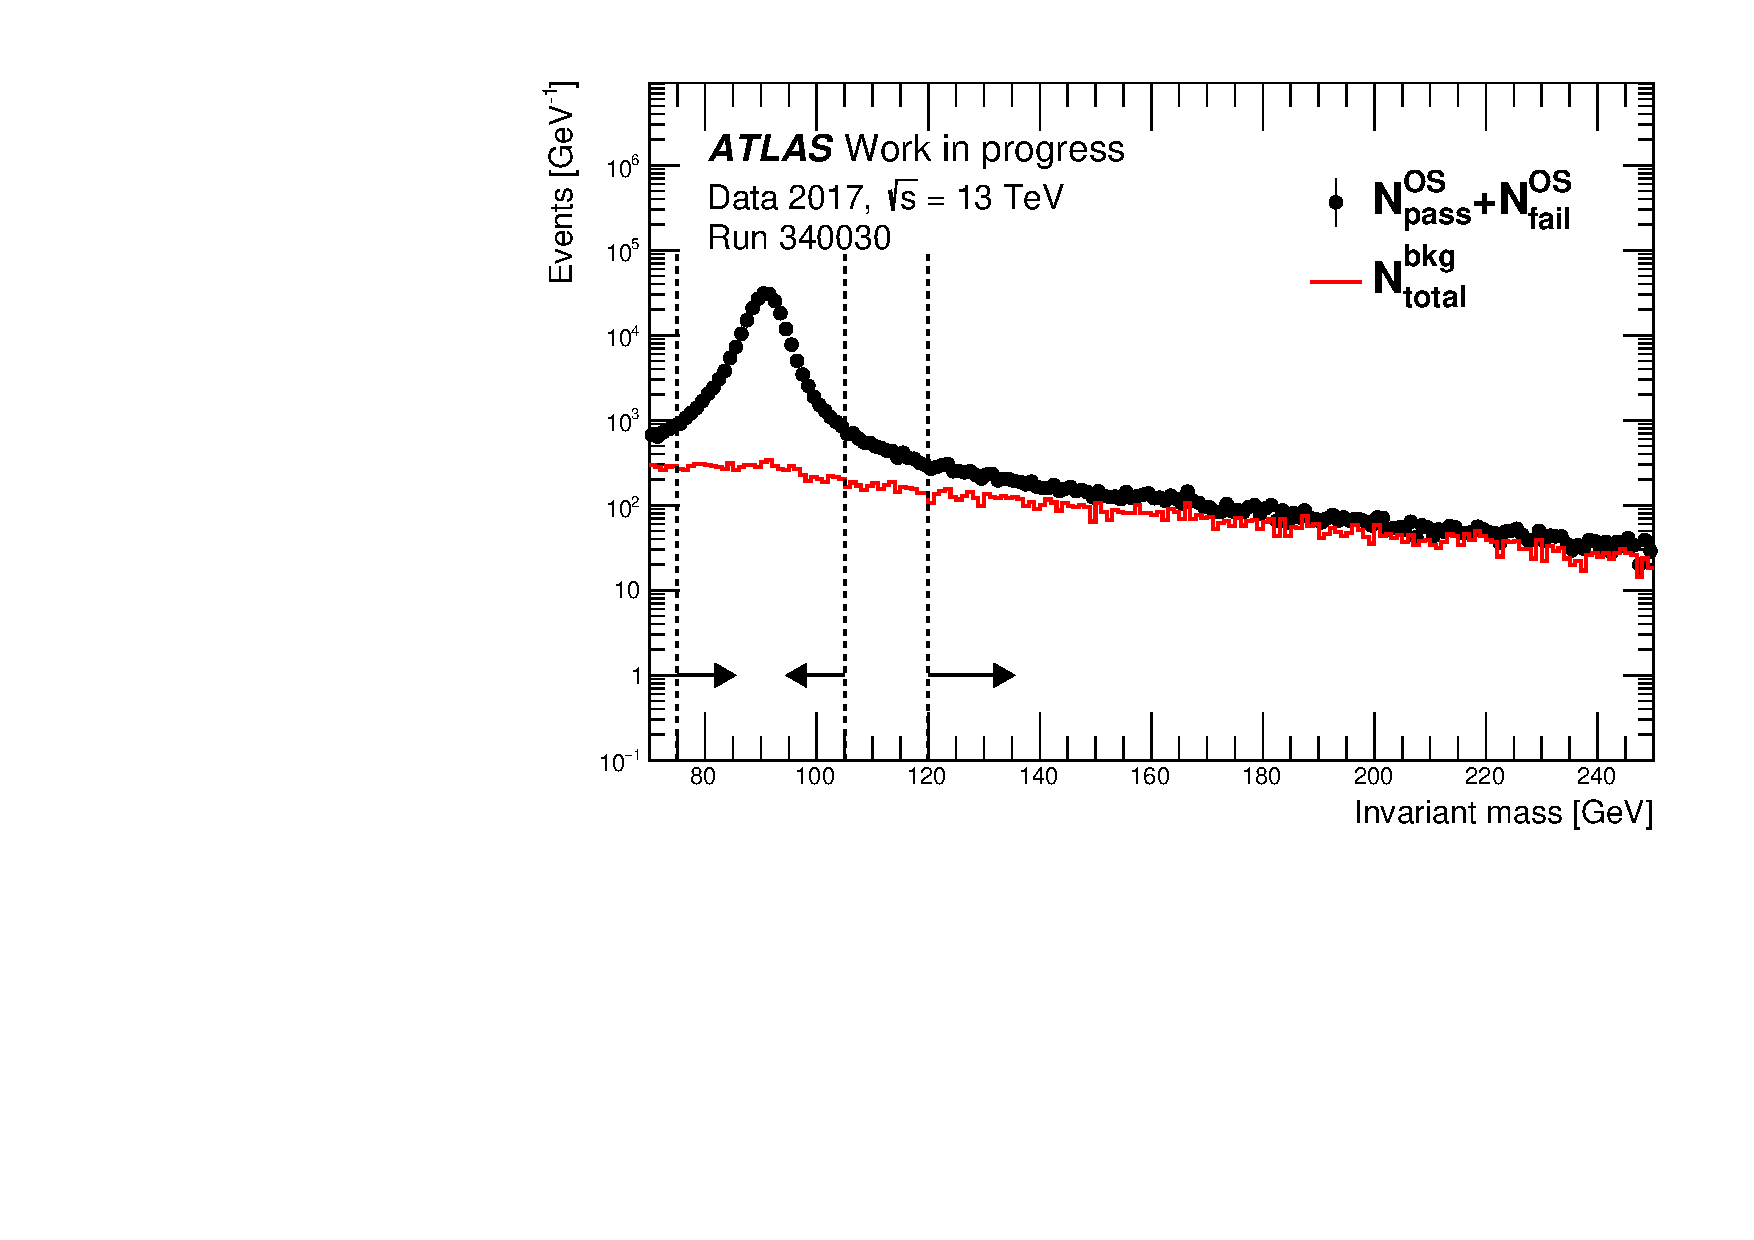
\includegraphics[width=0.48\textwidth]{figs/Zcount/TaP_Denominator_340030_ele.pdf}}
	\caption{Invariant dielectron mass distributions used to calculate the reconstruction efficiency as given in Eq.~\ref{eq:Zcount:Single-lep reco eff}, where the left(right) figure shows the contribution to the numerator (denominator). Vertical dashed lines illustrate the "peak" and "tail" mass ranges for the electron template method. The data was recorded from $pp$ collisions at $\sqrt{s}=13$~TeV in LHC Run 340030 on November 4, 2017. The error bars show statistical uncertainties only.}
	\label{fig:Zcount:Ele tag-and-probe}
\end{figure}

\begin{figure}[!htb]
	\centering
	\subfloat{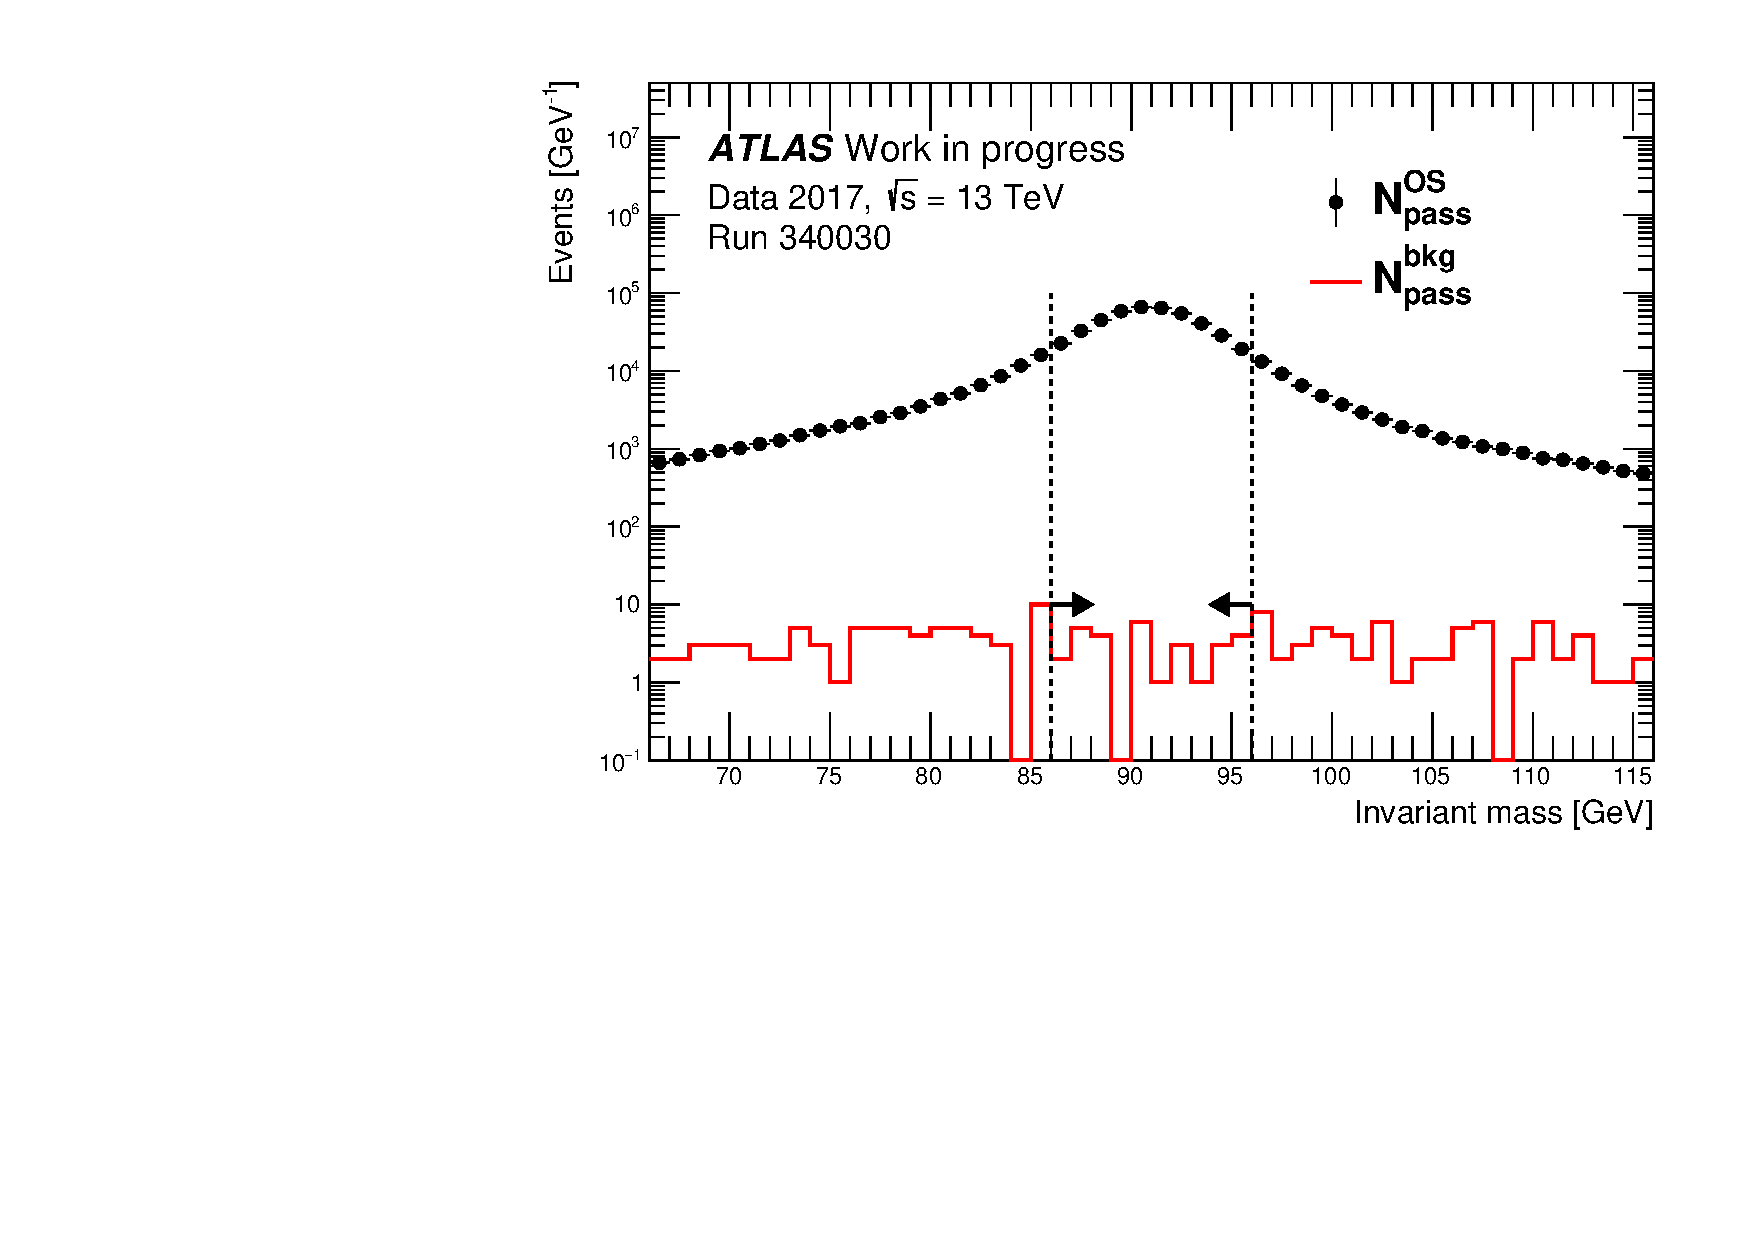
\includegraphics[width=0.48\textwidth]{figs/Zcount/TaP_Numerator_340030_muon.pdf}}
	\subfloat{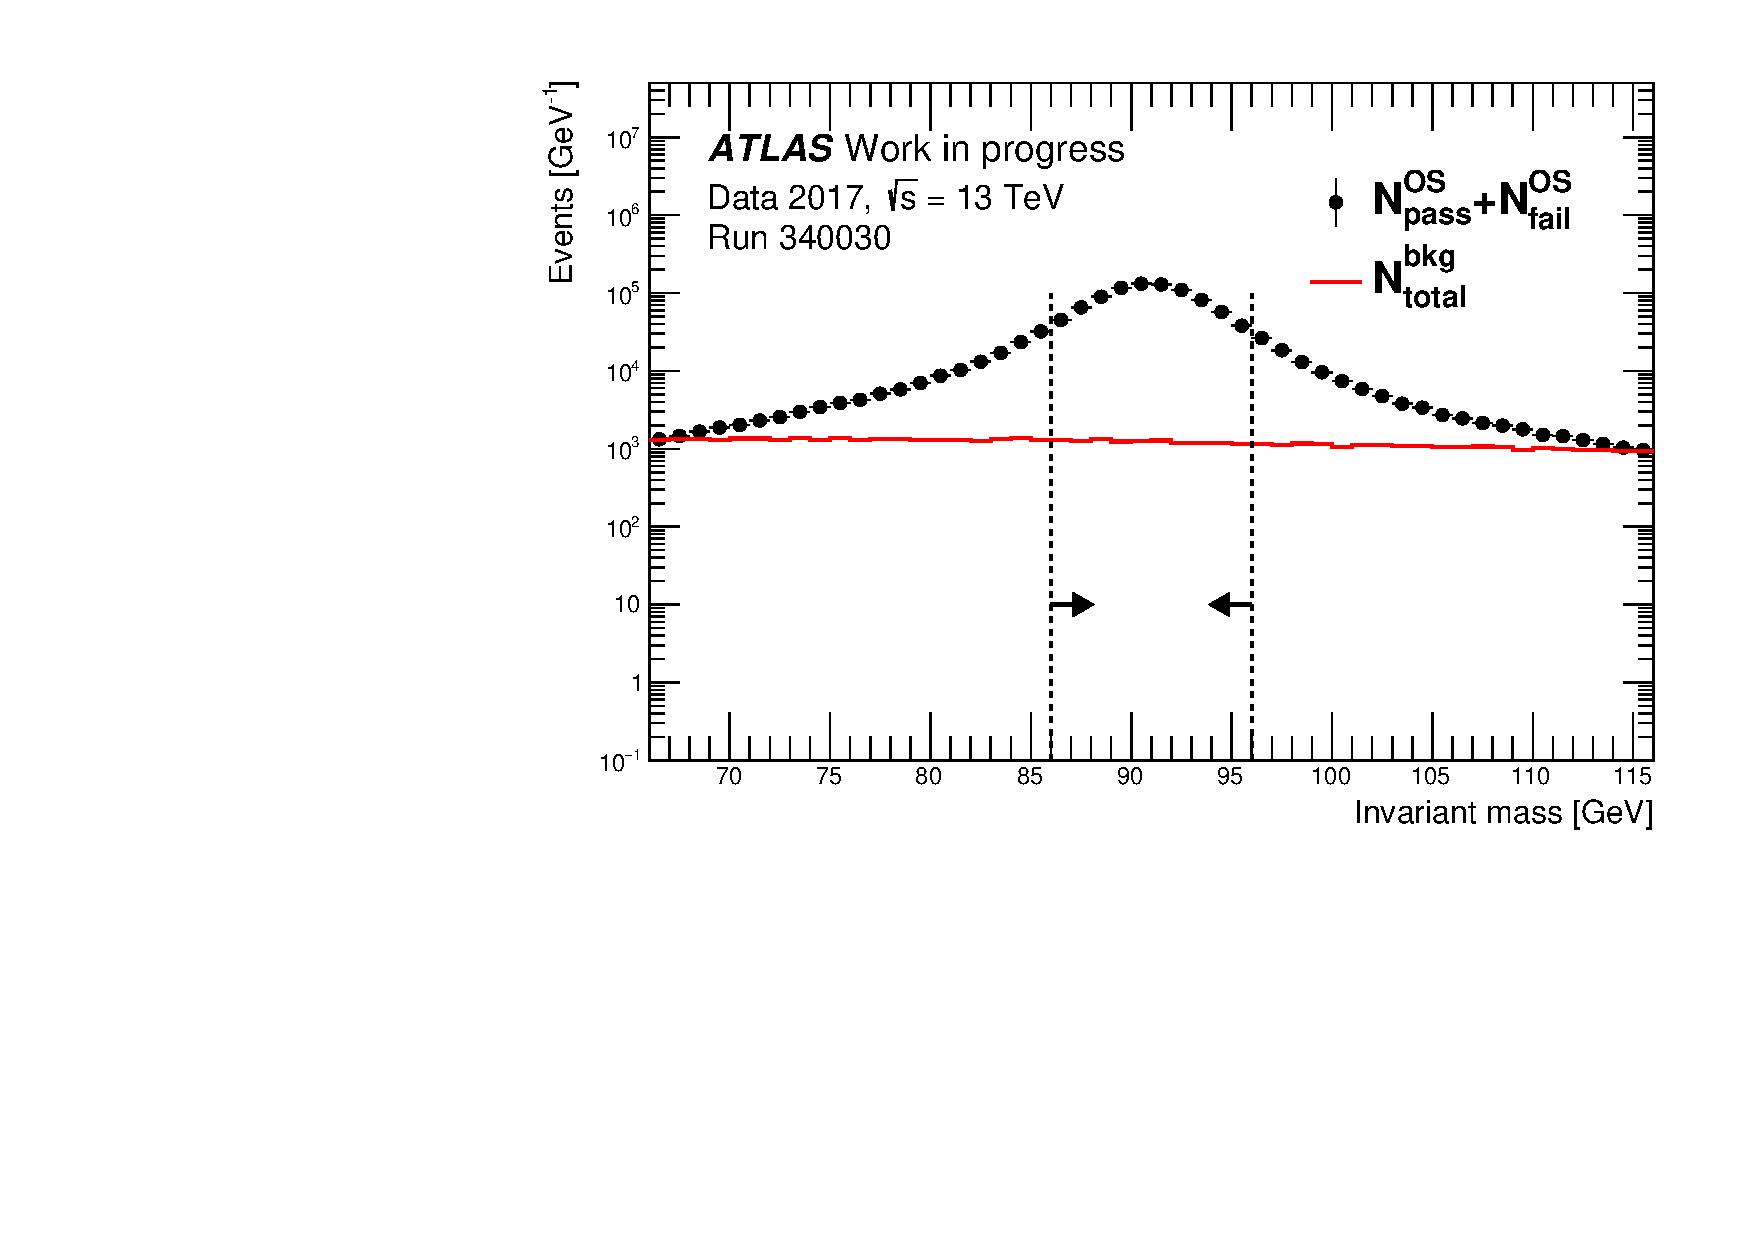
\includegraphics[width=0.48\textwidth]{figs/Zcount/TaP_Denominator_340030_muon.pdf}}
	\caption{Invariant dimuon mass distributions used to calculate the reconstruction efficiency as given in Eq.~\ref{eq:Zcount:Single-lep reco eff}, where the left(right) figure shows the contribution to the numerator (denominator). Vertical dashed lines illustrate the "peak" mass range used in the muon channel tag-and-probe procedure. The data was recorded from $pp$ collisions at $\sqrt{s}=13$~TeV in LHC Run 340030 on November 4, 2017. The error bars show statistical uncertainties only.}
	\label{fig:Zcount:Muon tag-and-probe}
\end{figure}

\subsubsection{Event-level efficiency}

For a $Z\rightarrow\ell^+\ell^-$ event there are two leptons and the single-lepton efficiencies are combined to determine event-level efficiencies. This considers that at least one lepton trigger the $Z$-candidate event and both lepton are required to pass the "good" lepton criteria:

\begin{equation}
	\varepsilon^\text{T\&P}_{Z\rightarrow \ell\ell}=\left( 1 - (1-\varepsilon_{\text{trig,}1\ell})^2 \right)\times\varepsilon^2_{\text{reco},1\ell}
	\label{eq:Zcount:Event level eff}
\end{equation}

The event-level efficiency, $\varepsilon^\text{T\&P}_{Z\rightarrow \ell\ell}$, is applied per decay channel to correct the number of raw $Z\rightarrow\ell^+\ell^-$ candidates. The corresponding statistical uncertainty is calculated by propagating the uncertainties on each component. The even-level efficiency is further corrected using a pileup-dependent correction factor derived from Monte Carlo, $F^\text{MC}_{Z\rightarrow \ell^+\ell^-}(\left< \mu \right>)$, which is the subject of Section~\ref{sec:Zcount:MC correction factor}.

\subsection{Correction factors from simulation}
\label{sec:Zcount:MC correction factor}

The event-level efficiency described in Eq.~\ref{eq:Zcount:Event level eff} accounts for the trigger and reconstruction efficiencies determined from data using a factorised ansatz based on single lepton efficiencies. However, it does not include additional effects due to the ID track efficiency for muons, nor the track-to-cluster matching efficiency and the electron charge mis-identification probability for electrons. Also, non-factorising effects are not included and could lead to a bias in the calculated event-level efficiency, due to the fact that the efficiencies of the two leptons may be correlated. This section outlines how the factorisation is tested and how a correction factor is obtained from samples of simulated $Z/\gamma^*\rightarrow\ell^+\ell^-$ events using the full ATLAS detector simulation.

\subsubsection{Samples and procedure}

The Monte Carlo $Z/\gamma^*\rightarrow\ell^+\ell^-$ signal samples used for this analysis are generated using Powheg~\cite{Nason:2004rx, Frixione:2007vw} for the hard scattering and Pythia8~\cite{Sjostrand:2014zea} using the AZNLO tune~\cite{ATLAS:2014alx} for the subsequent fragmentation and hadronisation. The effect of multiple $pp$ interactions in the same and neighbouring bunch crossings (pileup) is modelled by overlaying the hard-scattering event with simulated minimum-bias events generated with Pythia8.186 using the NNPDF2.3LO set of PDFs~\cite{Ball:2012cx} and the A3 tune~\cite{ATL-PHYS-PUB-2016-017}. The pileup profile with which the Monte Carlo is generated corresponds approximately to that of the data. The $Z$-signal samples are generated inclusively for true lepton pair masses of $m_{\ell^+\ell^-}>60$~GeV. The total efficiency times acceptance per channel is obtained from the fraction of simulated events in the sample that are successfully reconstructed at the detector level and pass the kinematic selection requirements shown in Table~\ref{tab:Zcount:LeptonSele}. The closure of the tag-and-probe procedure can then be tested by comparing the full reconstruction efficiency determined in Monte Carlo to the value of $\varepsilon^\text{T\&P}_{Z\rightarrow \ell\ell}$ determined using the tag-and-probe method on the Monte Carlo events.

The Monte Carlo correction factor, first introduced in Eq.~\ref{eq:Zcount:ZLumi_app}, $F^\text{MC}_{Z\rightarrow \ell^+\ell^-}(\left< \mu \right>)$, is defined as:

\begin{equation}
	F^\text{MC}_{Z\rightarrow \ell^+\ell^-}(\left< \mu \right>) = \frac{N^\text{reco,fid,MC}_{Z\rightarrow \ell^+\ell^-}(\left< \mu \right>)}{N^\text{true,nocut,MC}_{Z\rightarrow \ell^+\ell^-}(\left< \mu \right>)}\times\frac{1}{A^\text{MC}_{Z\rightarrow \ell^+\ell^-}\cdot \varepsilon^\text{T\&P,MC}_{Z\rightarrow \ell^+\ell^-}(\left< \mu \right>)}
	\label{eq:Zcount:MC factor}
\end{equation}

where all quantities are evaluated with Monte Carlo events as a function of the pileup parameter, $\left< \mu \right>$, and

\begin{itemize}
	\item $N^\text{reco,fid,MC}_{Z\rightarrow \ell^+\ell^-}(\left< \mu \right>)$ is the number of reconstructed events ("reco") which pass the fiducial phase space ("fid") and event selection requirements presented in Section~\ref{sec:Zcount:Event selection}.
	\item $N^\text{true,nocut,MC}_{Z\rightarrow \ell^+\ell^-}(\left< \mu \right>)$ is the number of generated $Z$ boson MC events ("true") without any selection ("nocut").
	\item $A^\text{MC}_{Z\rightarrow \ell^+\ell^-}$ is the fiducial acceptance, calculated using leptons originating from a $Z$ boson as described in Section~\ref{sec:Zcount:acceptance MC}.
	\item $\varepsilon^\text{T\&P,MC}_{Z\rightarrow \ell^+\ell^-}(\left< \mu \right>)$ is derived by repeating the tag-and-probe (T\&P) procedure using reconstructed MC events with small modifications to the background subtraction discussed in Section~\ref{sec:Zcount:tag-and-probe MC}.
\end{itemize}

The luminosity calculation in Eq.~\ref{eq:Zcount:ZLumi_app} depends only on the product $A^\text{MC}_{Z\rightarrow \ell^+\ell^-}\cdot F^\text{MC}_{Z\rightarrow \ell^+\ell^-}$, and $A^\text{MC}_{Z\rightarrow \ell^+\ell^-}$ appears in the denominator of the definition of $F^\text{MC}_{Z\rightarrow \ell^+\ell^-}$. Hence, the determined luminosity is independent of the value of $A^\text{MC}_{Z\rightarrow \ell^+\ell^-}$. The separation of these two terms is a matter of convention intended to capture the detector effects in $F^\text{MC}_{Z\rightarrow \ell^+\ell^-}$, but the $Z$-counting results do not depend on this separation.

The fraction of the left hand side of Eq.~\ref{eq:Zcount:MC factor} can be also rewritten in the form of a "total acceptance times efficiency", determined from MC, and can be denoted as $A\varepsilon(\left< \mu \right>)$:

\begin{equation}
A\varepsilon(\left< \mu \right>) = \frac{N^\text{reco,fid,MC}_{Z\rightarrow \ell^+\ell^-}(\left< \mu \right>)}{N^\text{true,nocut,MC}_{Z\rightarrow \ell^+\ell^-}(\left< \mu \right>)}
\end{equation}

\begin{equation}
\text{thus giving} \; F^\text{MC}_{Z\rightarrow \ell^+\ell^-}(\left< \mu \right>) = \frac{A\varepsilon(\left< \mu \right>)}{A^\text{MC}_{Z\rightarrow \ell^+\ell^-}\cdot \varepsilon^\text{T\&P,MC}_{Z\rightarrow \ell^+\ell^-}(\left< \mu \right>)}
\end{equation}

The term $A\varepsilon$ can be thus seen as the product of a "pure" phase space acceptance $A$ and reconstruction efficiency effects due to the detector, $\varepsilon(\left< \mu \right>)$, which can depend on pileup. In general, it cannot be assumed that the two "factors" can be resolved, and $\varepsilon^\text{T\&P,MC}_{Z\rightarrow \ell^+\ell^-}$ may not capture all efficiency effects, therefore one cannot necessarily expect $F^\text{MC}_{Z\rightarrow \ell^+\ell^-}=1$ in practice.

\subsubsection{Fiducial acceptance}
\label{sec:Zcount:acceptance MC}

The acceptance factor $A^\text{MC}_{Z\rightarrow \ell^+\ell^-}$ is derived from the MC signal samples using true $Z$-boson events as follows

\begin{equation}
A^\text{MC}_{Z\rightarrow \ell^+\ell^-} =  \frac{N^\text{true,fid,MC}_{Z\rightarrow \ell^+\ell^-}}{N^\text{true,nocut,MC}_{Z\rightarrow \ell^+\ell^-}}
\end{equation}

where

\begin{itemize}
	\item $N^\text{true,fid,MC}_{Z\rightarrow \ell^+\ell^-}$ is the number of generated events with a pair of opposite-sign leptons with $p_\text{T}>27$~GeV, $|\eta|<2.4$ (with the additional removal of the crack region $1.37<|\eta|<1.52$ for electrons) and $66<m_{\ell\ell}<116$~GeV.
	\item $N^\text{true,nocut,MC}_{Z\rightarrow \ell^+\ell^-}$ is the number of generated events with a true mass of $m_{\ell\ell}>60$~GeV.
\end{itemize}

In order to yield residual factors, $F^\text{MC}_{Z\rightarrow \ell^+\ell^-}$, that are close to one, an appropriate definition of $A^\text{MC}_{Z\rightarrow \ell^+\ell^-}$ is needed. This is achieved by using \textit{bare} and \textit{dressed} definition\footnote{Further details on those definitions can be found in Ref.~\cite{ATLAS:2019zci}.} for the generator-level lepton kinematics for muon and electron channels, respectively. The \textit{bare} momentum corresponds to the lepton after emission of QED final state radiation (QED FSR) and is appropriate for muons, where the momentum is measured from the track. The \textit{dressed} mometum is obtained by combining the bare four-momenum with that of the radiated QED FSR photons within a cone of size $\Delta R =0.1$ around the lepton. This is appropriate for electrons, where the energy is measured in the electromagnetic calorimeter, as the photon and electron energy deposits overlap. The obtained acceptance values for $A^\text{MC}_{Z\rightarrow \ell^+\ell^-}$ are shown in Table~\ref{tab:Zcount:MC acceptance}. As previously mentioned, the calculation details of $A^\text{MC}_{Z\rightarrow \ell^+\ell^-}$ do not impact the final luminosity determination, therefore the uncertainties on this value are not considered.

\begin{table}[!htb]
	\centering
	\begin{tabular}{@{}cc@{}}
		\toprule
		$A^\text{MC}_{Z\rightarrow e^+e^-}$    & $A^\text{MC}_{Z\rightarrow \mu^+\mu^-}$    \\ \midrule
		$0.2996\pm0.0002$ & $0.3326\pm0.0002$ \\ \bottomrule
	\end{tabular}
	\caption{Fiducial acceptance values, calculated for the electron and muon channels using the corresponding MC signal samples. The uncertainties reflect the statistical uncertainty of the simulated data.}
	\label{tab:Zcount:MC acceptance}
\end{table}

\subsubsection{Tag-and-probe efficiency in Monte Carlo}
\label{sec:Zcount:tag-and-probe MC}

The pileup-dependent correction factor, $F^\text{MC}_{Z\rightarrow \ell^+\ell^-}(\left< \mu \right>)$, and its components are derived using Monte Carlo $Z/\gamma^*\rightarrow\ell^+\ell^-$ signal samples. This involves the full application of the efficiency measurement procedure detailed in Section~\ref{sec:Zcount:Data driven effs} for the data. As opposed to the analysis performed with data, each event contains a true $Z\rightarrow\ell\ell$ decay and there is no QCD multijet contamination. However, a small amount of background could be present in the tag-and-probe distributions due to misidentified hadronic activity, non-prompt lepton production and overlaid pileup events. This is removed by requiring the reconstructed leptons to be matched to a generated lepton from the $Z\rightarrow\ell\ell$ decay. In the muon channel it was verified that using generator level information yields compatible results obtained when using same-charge events. The single lepton efficiencies obtained with reconstructed MC events according to Equations~\ref{eq:Zcount:Single-lep trig eff} and \ref{eq:Zcount:Single-lep reco eff} are then combined in the same way as in data using Eq.~\ref{eq:Zcount:Event level eff} to an event-level $Z$ boson efficiency, $\varepsilon^\text{T\&P,MC}_{Z\rightarrow \ell^+\ell^-}(\left< \mu \right>)$.

\subsubsection{Results for the Monte Carlo correction factor}

Following the procedure aforementioned the pileup-dependent Monte Carlo correction factors, $F^\text{MC}_{Z\rightarrow \ell^+\ell^-}(\left< \mu \right>)$ are dervied. In order to properly model the different condition for each data-taking periods (each individual year between 2015 and 2018), correction factors are calculated separately using the corresponding Monte Carlo simulations.

The $\left< \mu \right>$ dependence of $F^\text{MC}_{Z\rightarrow \ell^+\ell^-}$ is fitted with a second-order polynomial per decay channel and per data-taking period, and the fit results are shown in Figure~\ref{fig:Zcount:MC correction factors}.

The $Z\rightarrow e^+e^-$ correction factor is >10\% below unity for all $\left< \mu \right>$, implying that there are additional efficiency effects beyond those captured in the tag-and-probe procedure. The variation between $\left< \mu \right>=20$ and $\left< \mu \right>=50$ is around 2\%, suggesting that pileup-dependent effects are mild.

\begin{figure}[!htb]
	\centering
	\subfloat{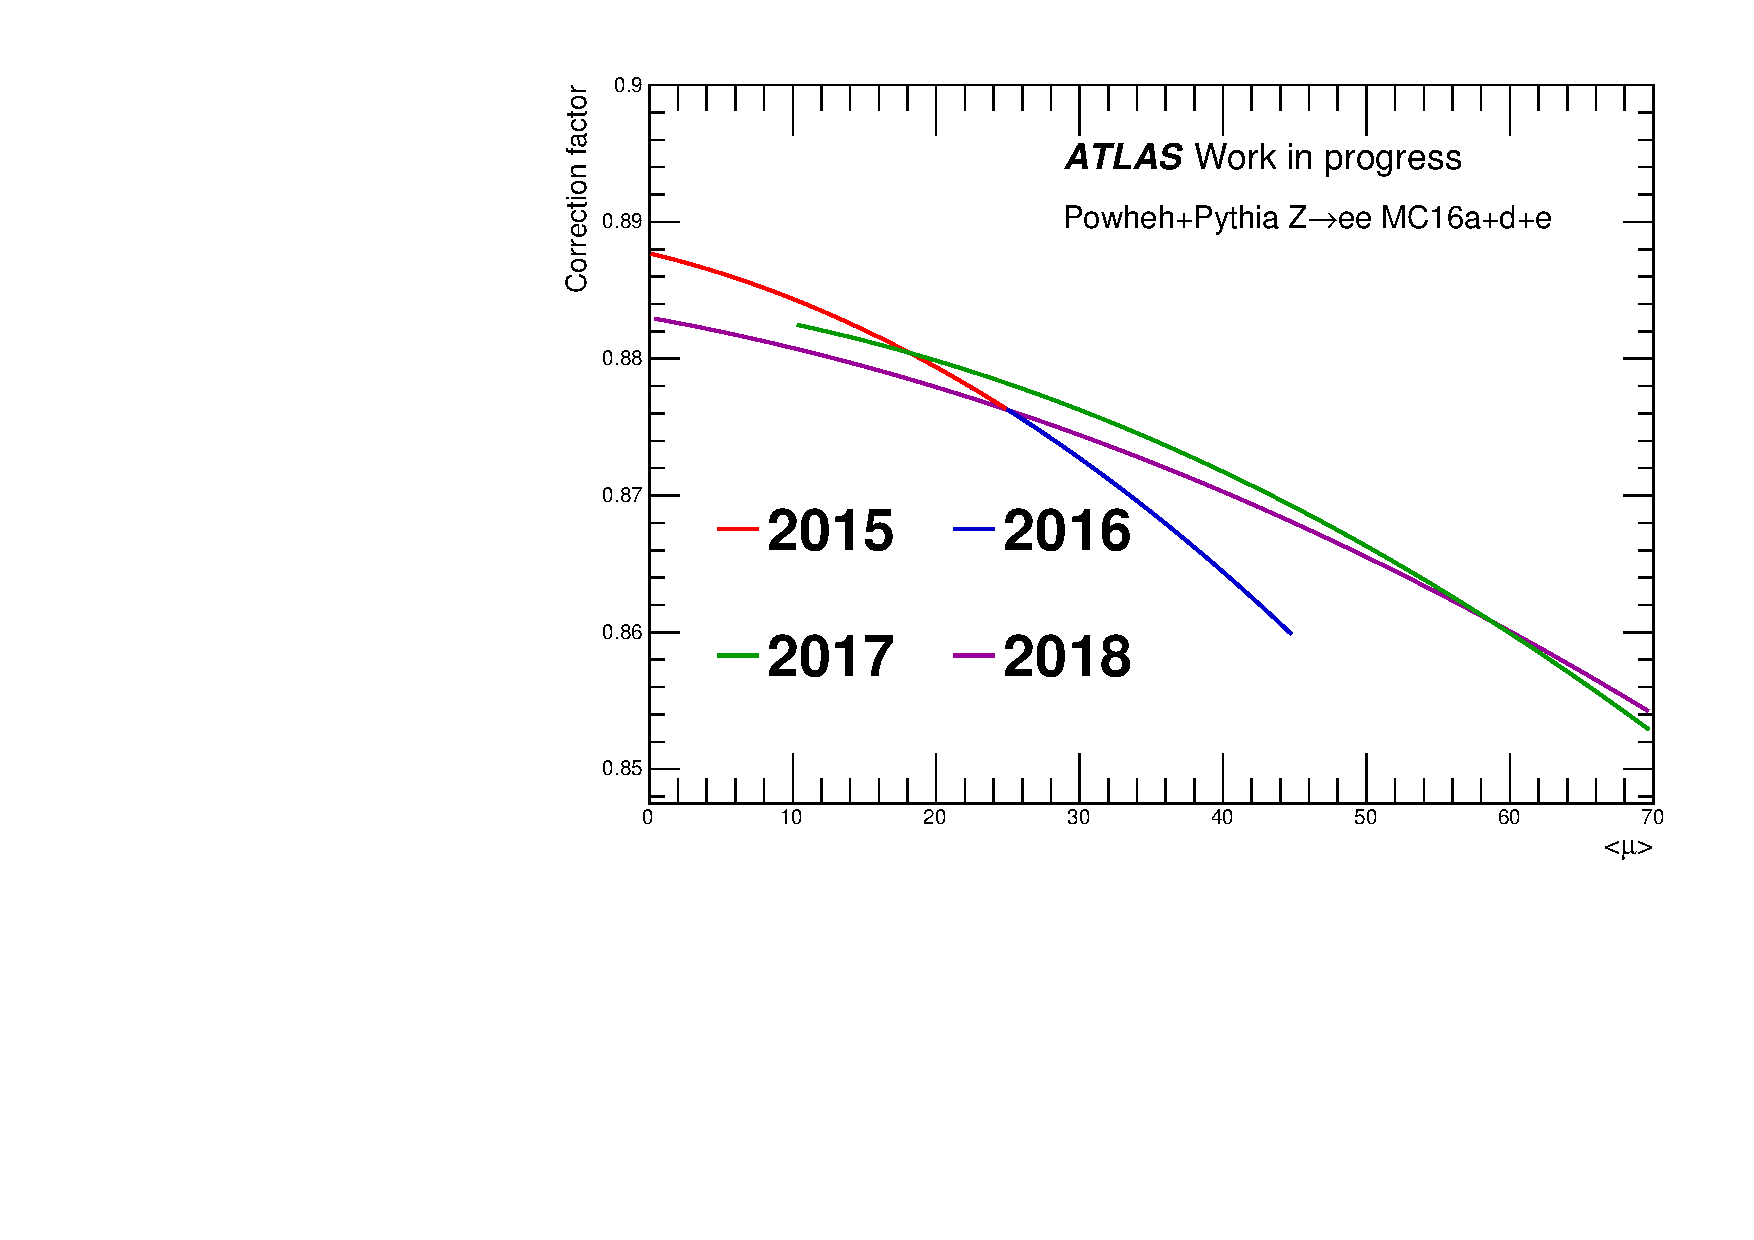
\includegraphics[width=0.48\textwidth]{figs/Zcount/YearlyFMC_ele.pdf}}
	%\subfloat{\includegraphics[width=0.48\textwidth]{figs/Zcount/YearlyFMC_mu.pdf}}
	\caption{$Z\rightarrow e^+e^-$ correction factors used for each year of data produced using the dedicated Monte Carlo campaigns. The lines show second-order polynomial fits to the correction factor for the corresponding $\left< \mu \right>$ range per year.}
	\label{fig:Zcount:MC correction factors}
\end{figure}

The fits of $F^\text{MC}_{Z\rightarrow \ell^+\ell^-}$, as shown in Figure~\ref{fig:Zcount:MC correction factors}, are used in the determination of the Z-counting based luminosity per data-taking period and as a function of the pileup parameter $\left< \mu \right>$. The statistical uncertainties of the fits are small and are neglected.

\subsection{Results}

\subsubsection{Results in a typical LHC run}

The results of each of the steps to perform a Z-counting based luminosity measurement are illustrated using ATLAS data taken in typical LHC runs. As shown in Table~\ref{tab:Zcount:Example runs}, the $pp$ luminosity delivered per run, as well as the average number of interactions per bunch crossing, increased significantly from year to year. The following section shows detailed results illustrating the methodology of $Z$-counting using data recorded for $\sqrt{s}=13$~TeV $pp$ collisions in LHC runs 281411, 300800, 340030 and 360373 on 2015, 2016, 2017 and 2018 respectively.

\begin{table}[!htb]
	\centering
	\begin{tabular}{@{}ccccc@{}}
		\toprule
		Data-taking period & LHC Run & Date     & Luminosity [pb$^{-1}$] & Average pileup $\left< \mu \right>$ \\ \midrule
		2015               & 281411  & 11/10/15 & 163.5         & 15.1           \\
		2016               & 300800  & 03/06/16 & 313.0         & 21.8           \\
		2017               & 340030  & 04/11/17 & 725.3         & 39.9           \\
		2018               & 360373  & 09/09/18 & 416.8         & 37.5           \\ \bottomrule
	\end{tabular}
	\caption{Information for the selected LHC fills used to illustrate the Z-counting methodology for each of the Run-2 data-taking periods.}
	\label{tab:Zcount:Example runs}
\end{table}

The single-lepton reconstruction and trigger efficiencies for each of these runs are shown in Figure~\ref{fig:Zcount:Single-electron efficiencies}. Furthermore, the Z-counting based luminosity is compared to the baseline ATLAS luminosity value for the $\sqrt{s}=13$~TeV proton-proton dataset~\cite{ATLAS-CONF-2019-021} in Figure~\ref{fig:Zcount:Single run lumi electron}. Due to the sensitivity of the $Z$ cross-section to the details of the proton structure function, the absolute ratio has to be the subject of a dedicated, high precision physics analysis and will be not discussed further here. It is noted that this ratio is consistent with unity within the total uncertainty when adding the dominant theoretical and experimental systematic uncertainties in quadrature. The remainder of the present note focuses on the relative consistency of the $Z$-counting and baseline ATLAS luminosity measurements, primarily as a function of time.

Therefore, in all comparison of the $Z$-counting and baseline luminosities, the $Z$-counting luminosity is normalised to the same integrated luminosity as the baseline ATLAS measurement. This can be done over different time periods, for instance a single LHC Run, a single-data taking period (year) or the entire Run 2 period. By normalising the $Z$-counting luminosity in this way, the relative stability of the baseline ATLAS luminosity can be monitored independently of the absolute scale of the $Z$-counting measurmeent. It is also a useful diagnostic tool to detect trends, such as changes in LHC running conditions.

The data-driven single-lepton efficiencies are shown in Figure~\ref{fig:Zcount:Single-electron efficiencies}. For these figures, the efficiencies have been obtained by a weighted average over 20 luminosity blocks to improve the statistical prediction for display purposes. The efficiencies track the variation of the lepton detection across the Run, with efficiencies reflecting the time evolution of actual data-taking conditions.

After forming the $Z$ event-level efficiencies and applying the pileup-dependent Monte Carlo correction factors per LB, $Z$-counting luminosities are combined for 20 LBs, as, 

\begin{equation}
\mathcal{L_{Z\rightarrow \ell^+\ell^-}} = \frac{\sum_{LB}^{N}L_{Z\rightarrow \ell^+\ell^-}(LB)\cdot t(LB)}{\sum_{LB}^{N} t(LB)}
\end{equation}

where $L_{Z\rightarrow \ell^+\ell^-}(LB)$ is the individual $Z$-counting luminosity for each LB and $t(LB)$ is the duration of said luminosity block.

To monitor the stability of the luminosity per run, the $Z$-counting luminosity is normalised to the run-integrated baseline ATLAS luminosity, obtaining the results shown in Figure~\ref{fig:Zcount:Single run lumi electron}. The ratio of the normalised $Z$-counting and ATLAS luminosities has a spread at or below the 2\% level, indicating the excellent stability of the $Z$-counting methodology.

\begin{figure}[!htb]
	\centering
	\subfloat{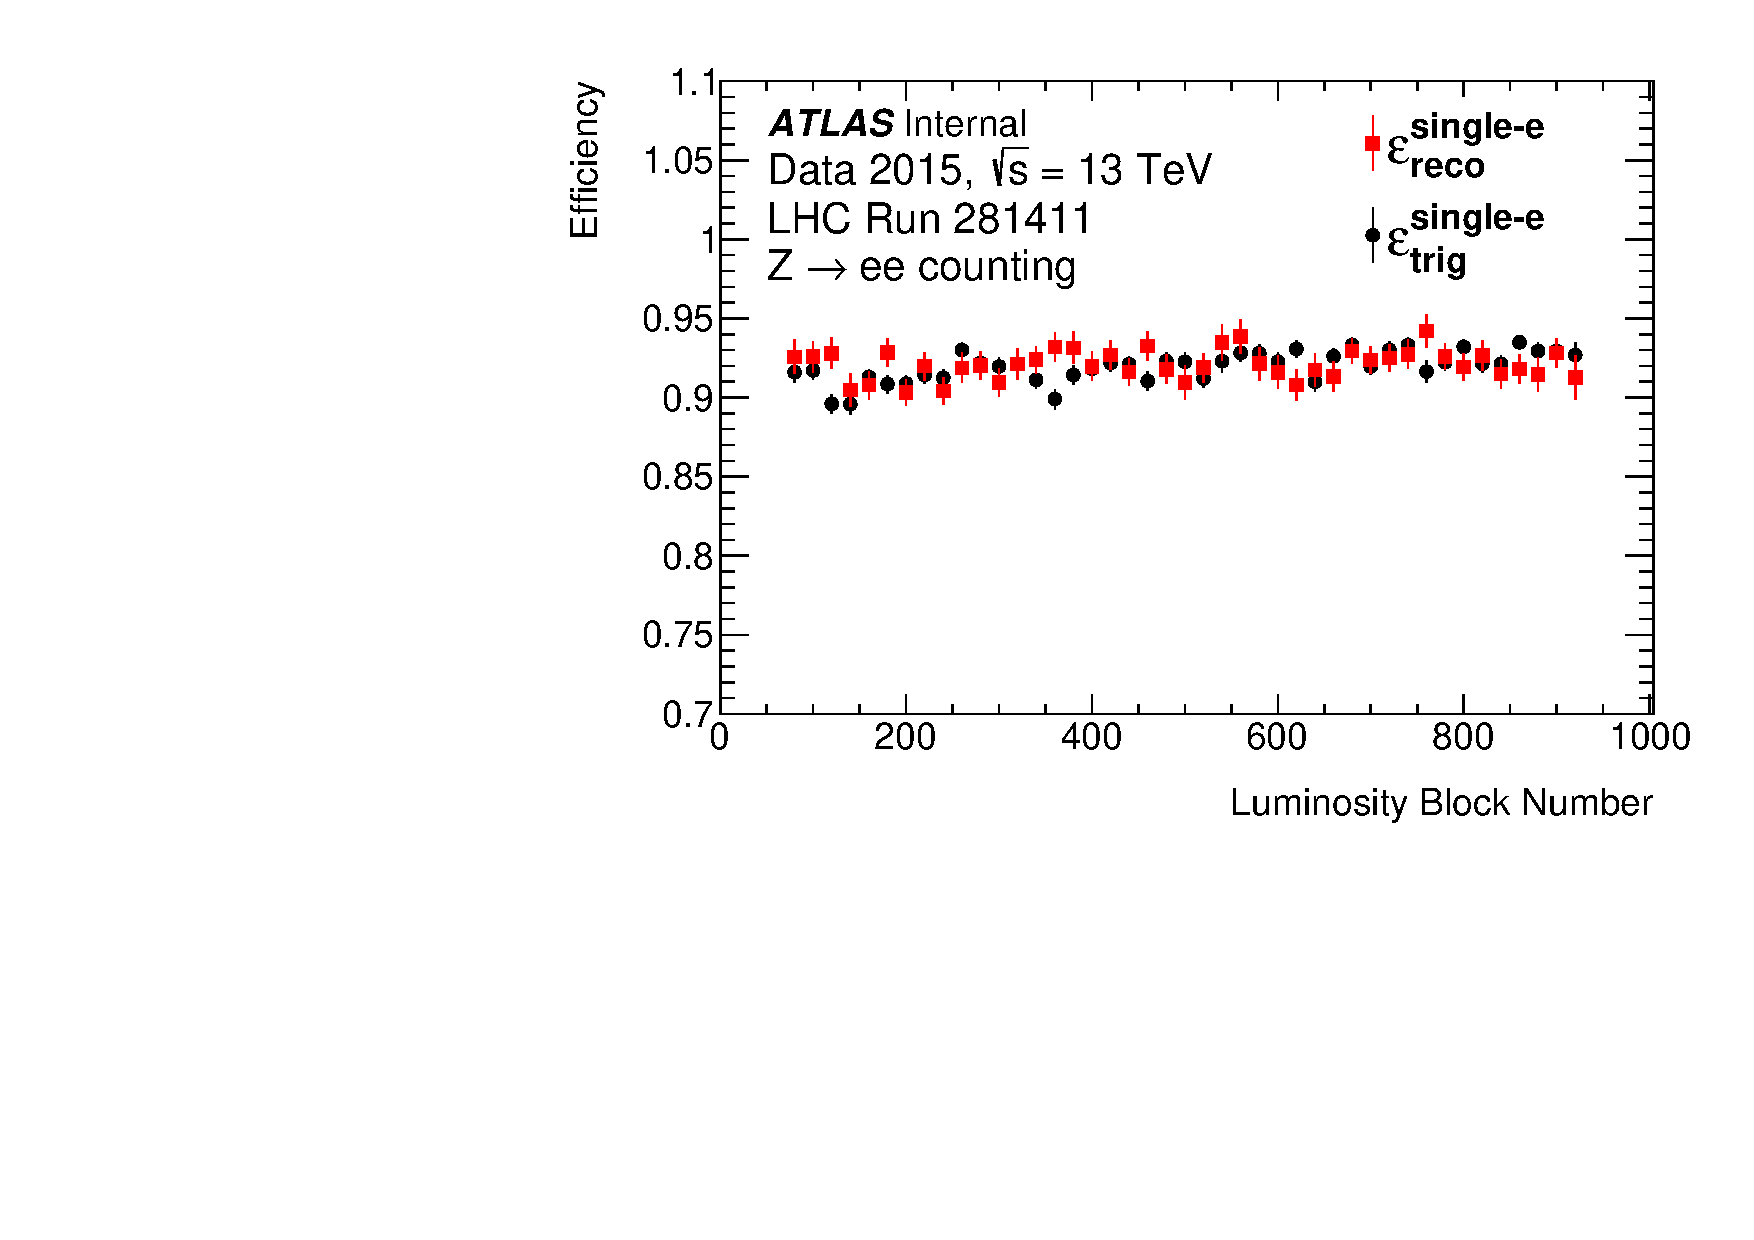
\includegraphics[width=0.48\textwidth]{figs/Zcount/Effs/eff_v_lb_Zee_data15_281411.pdf}}
	\subfloat{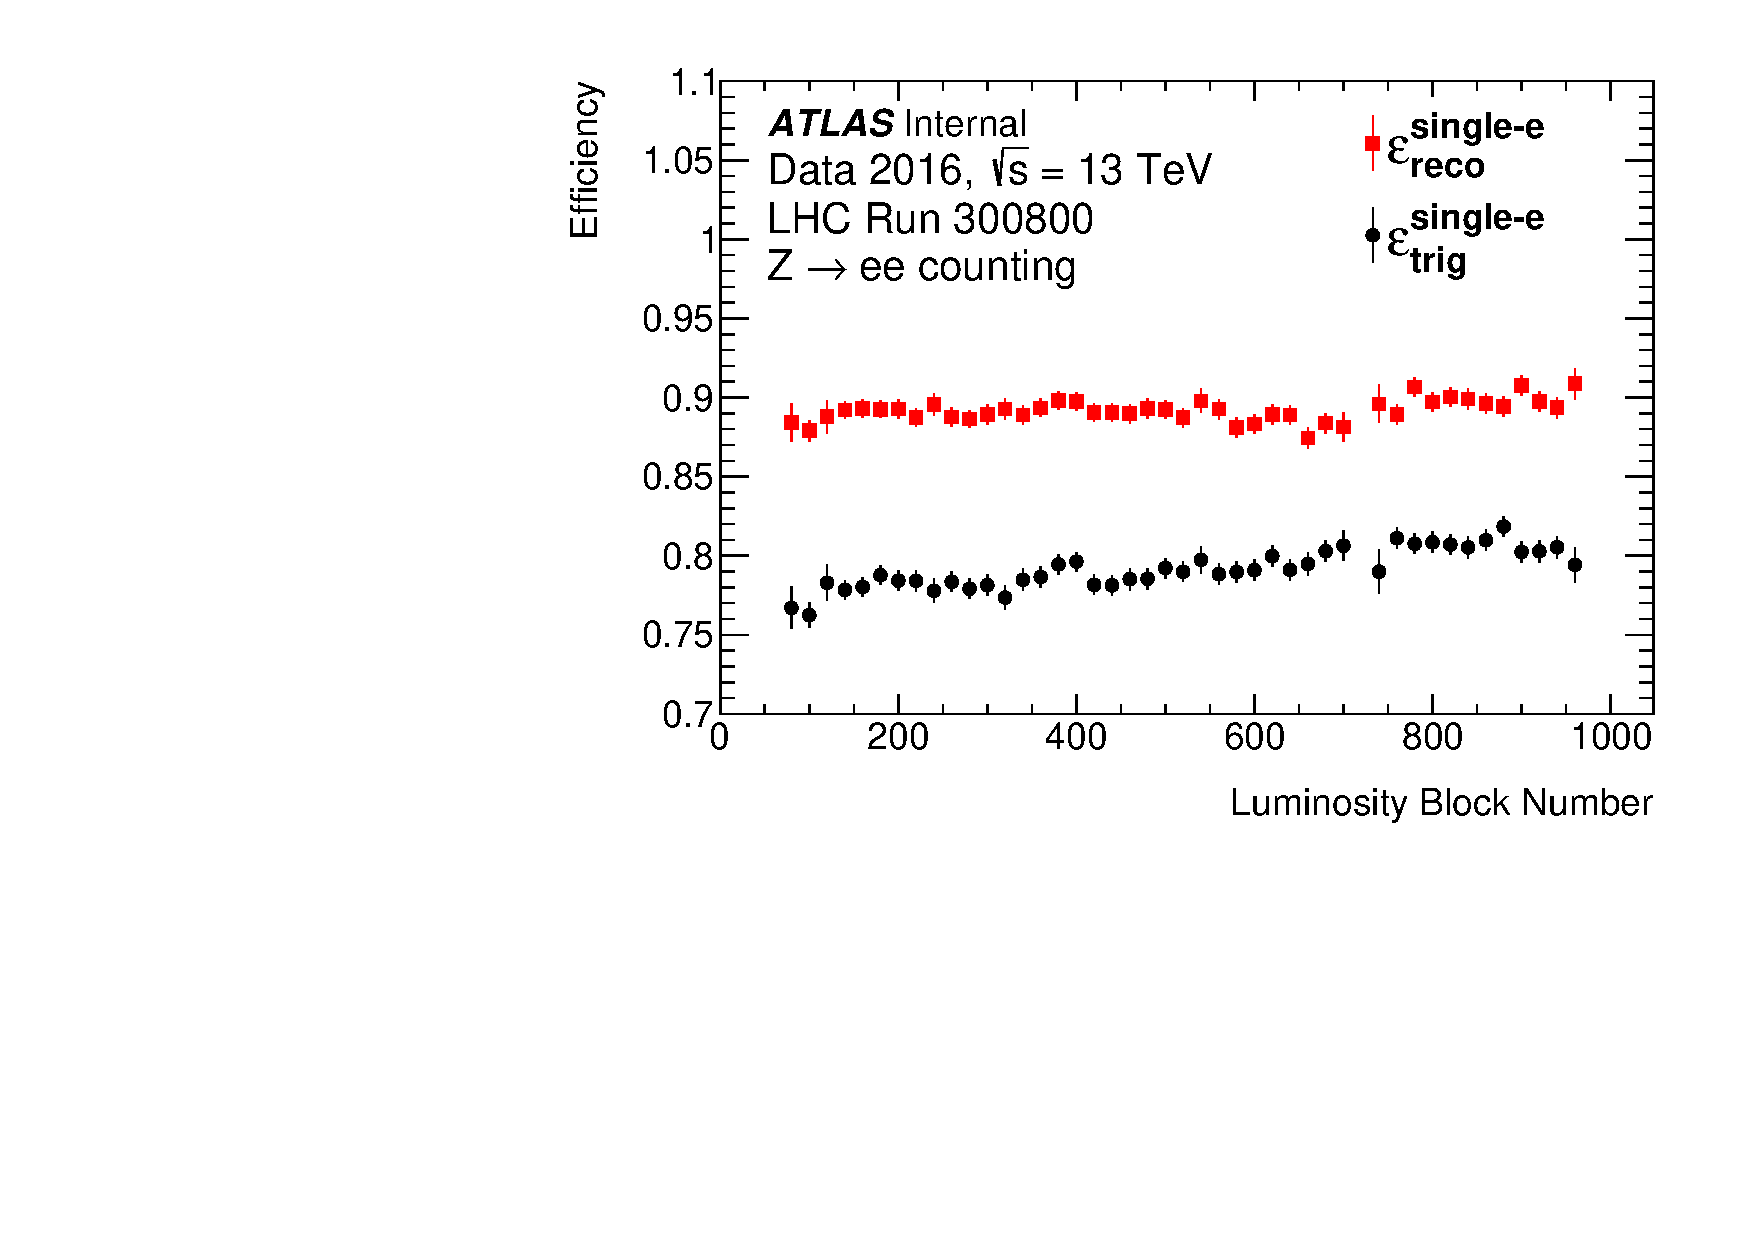
\includegraphics[width=0.48\textwidth]{figs/Zcount/Effs/eff_v_lb_Zee_data16_300800.pdf}}\\
	\subfloat{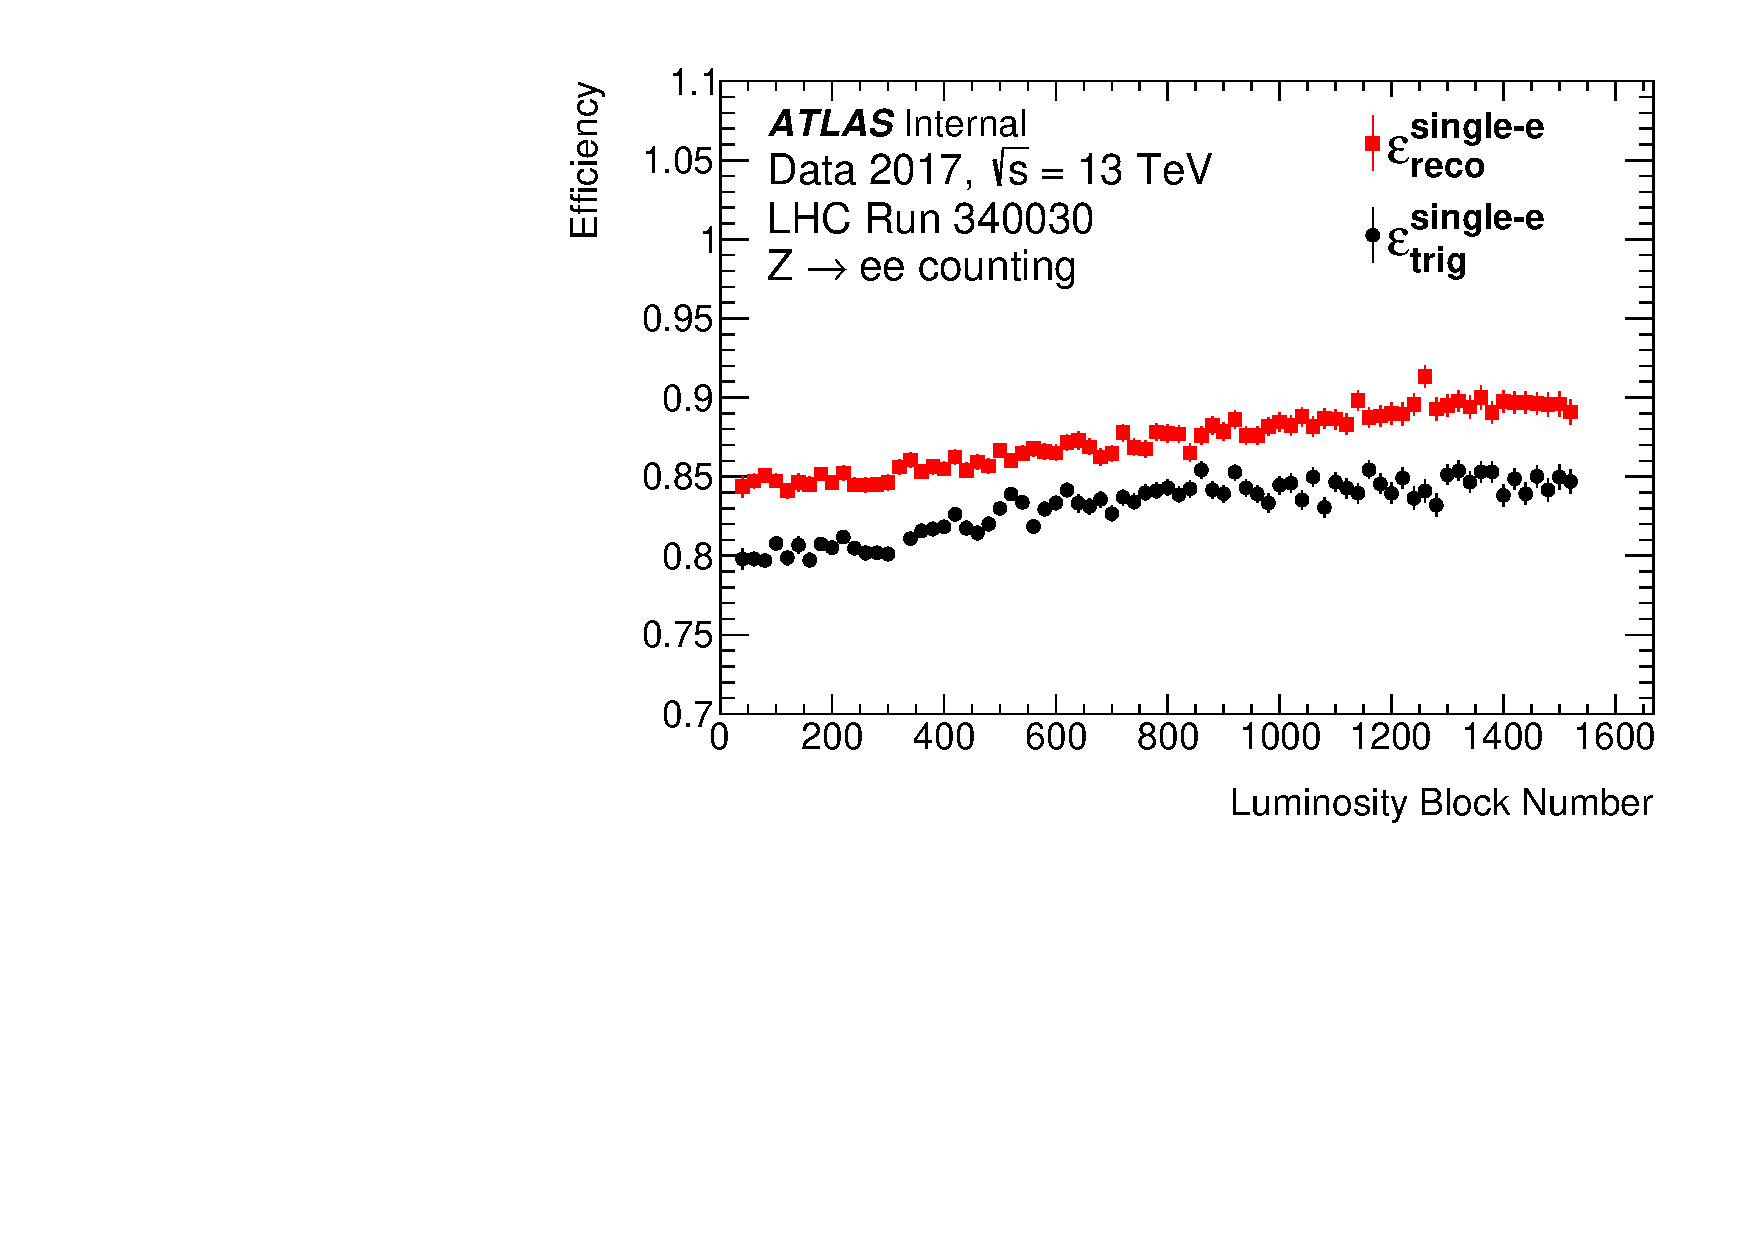
\includegraphics[width=0.48\textwidth]{figs/Zcount/Effs/eff_v_lb_Zee_data17_340030.pdf}}
	\subfloat{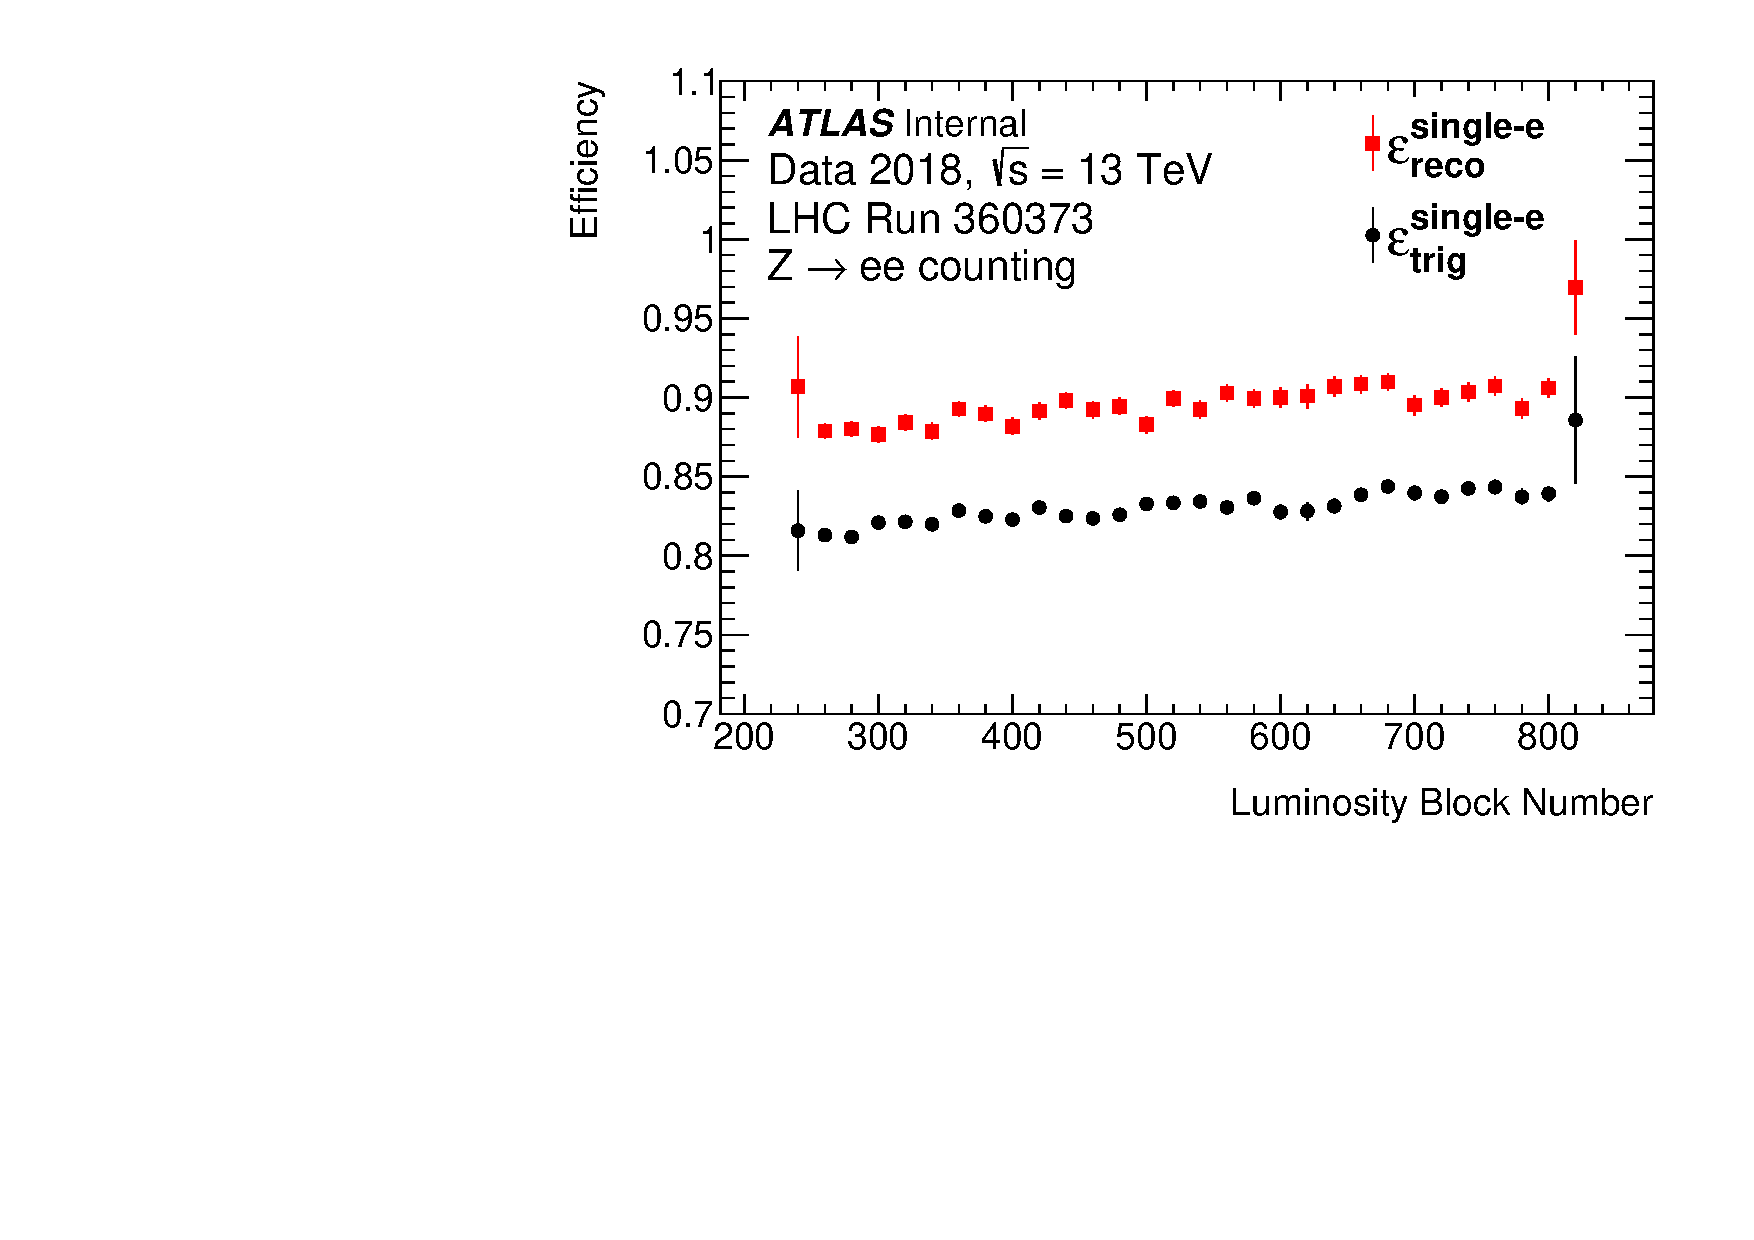
\includegraphics[width=0.48\textwidth]{figs/Zcount/Effs/eff_v_lb_Zee_data18_360373.pdf}}
	\caption{Time-dependence of the data-driven single electron trigger (black circles) and reconstruction (red square) efficiencies in each data-taking period. Efficiencies were determined using the tag-and-probe method, as explained in Section~\ref{sec:Zcount:Data driven effs}, and shown is the average of the quantities over 20 luminosity blocks. Error bars show statistical uncertainties.}
	\label{fig:Zcount:Single-electron efficiencies}
\end{figure}

\begin{figure}[!htb]
	\centering
	\subfloat{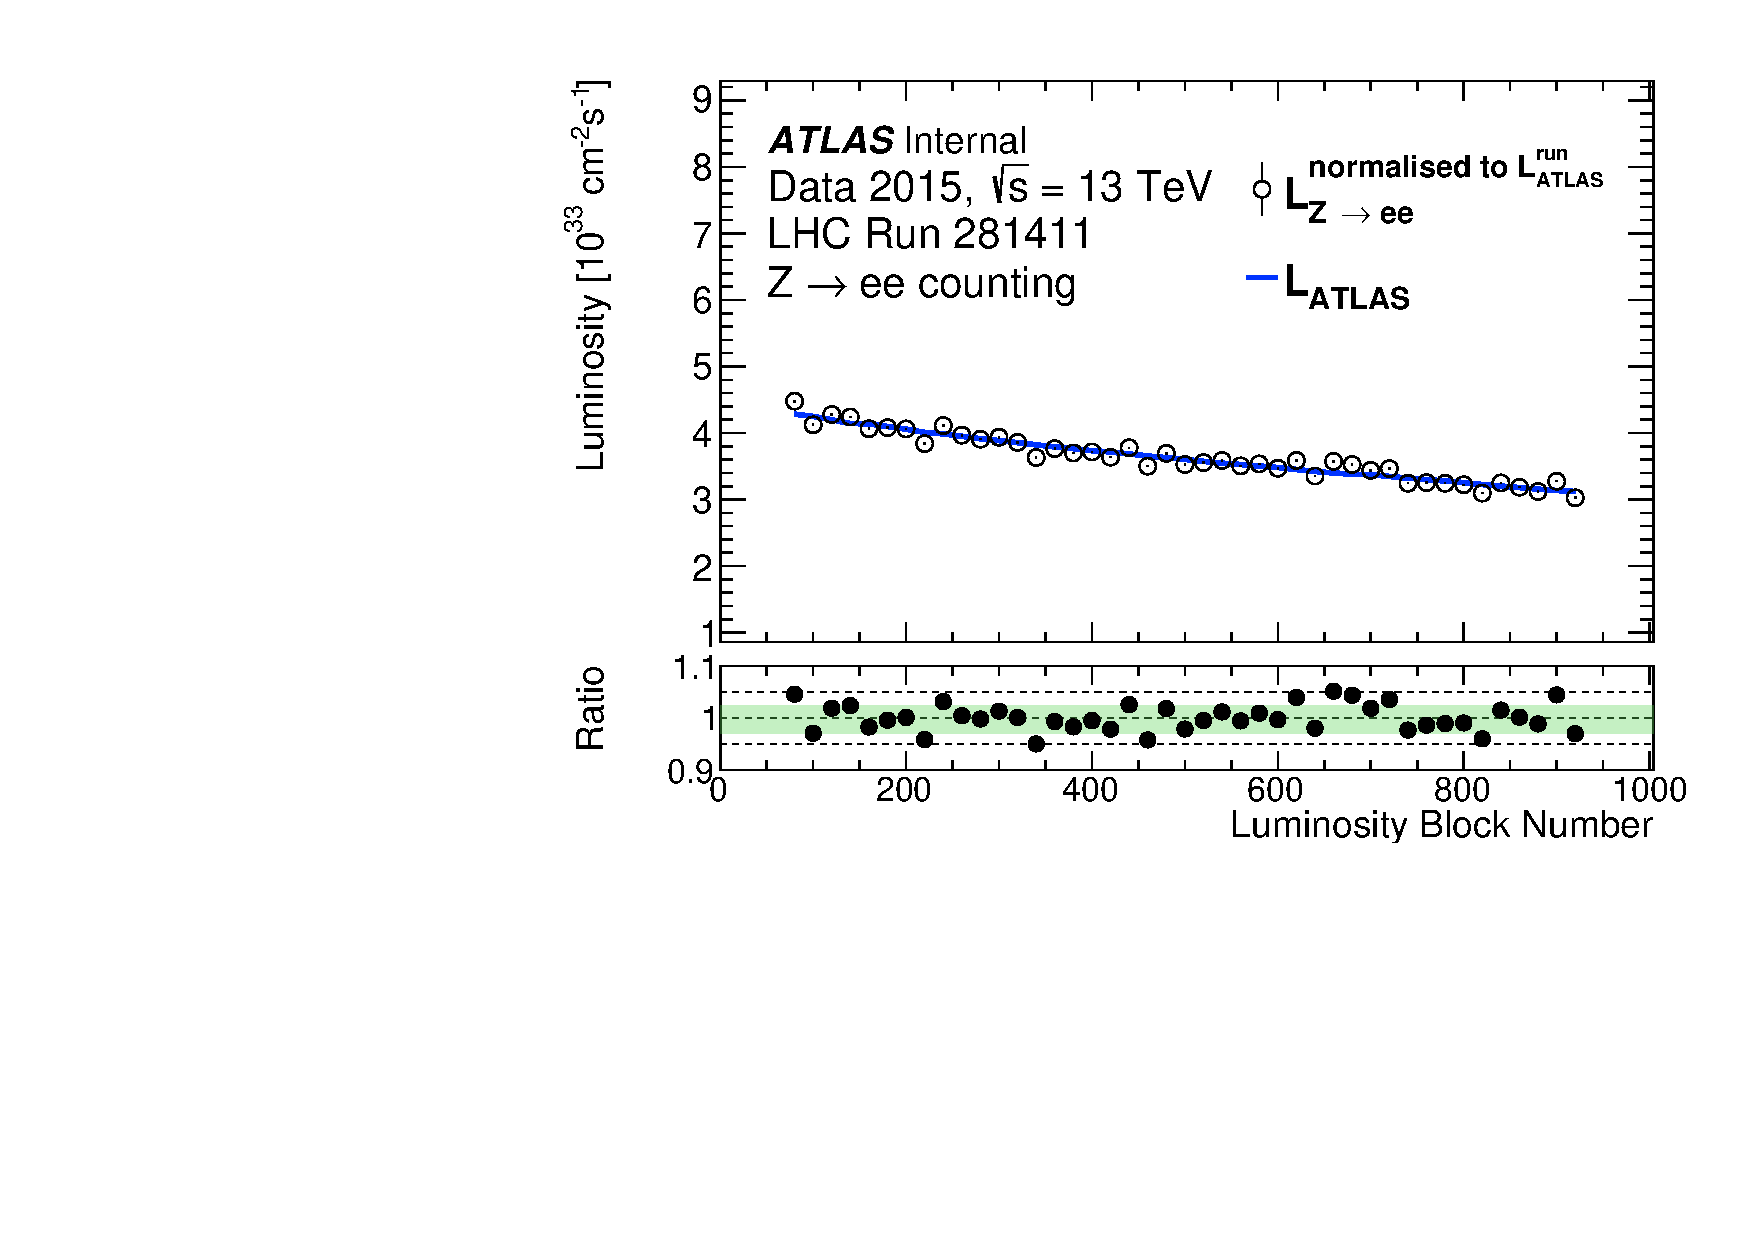
\includegraphics[width=0.48\textwidth]{figs/Zcount/Lumi/281411_Zee_vs_atlas.pdf}}
	\subfloat{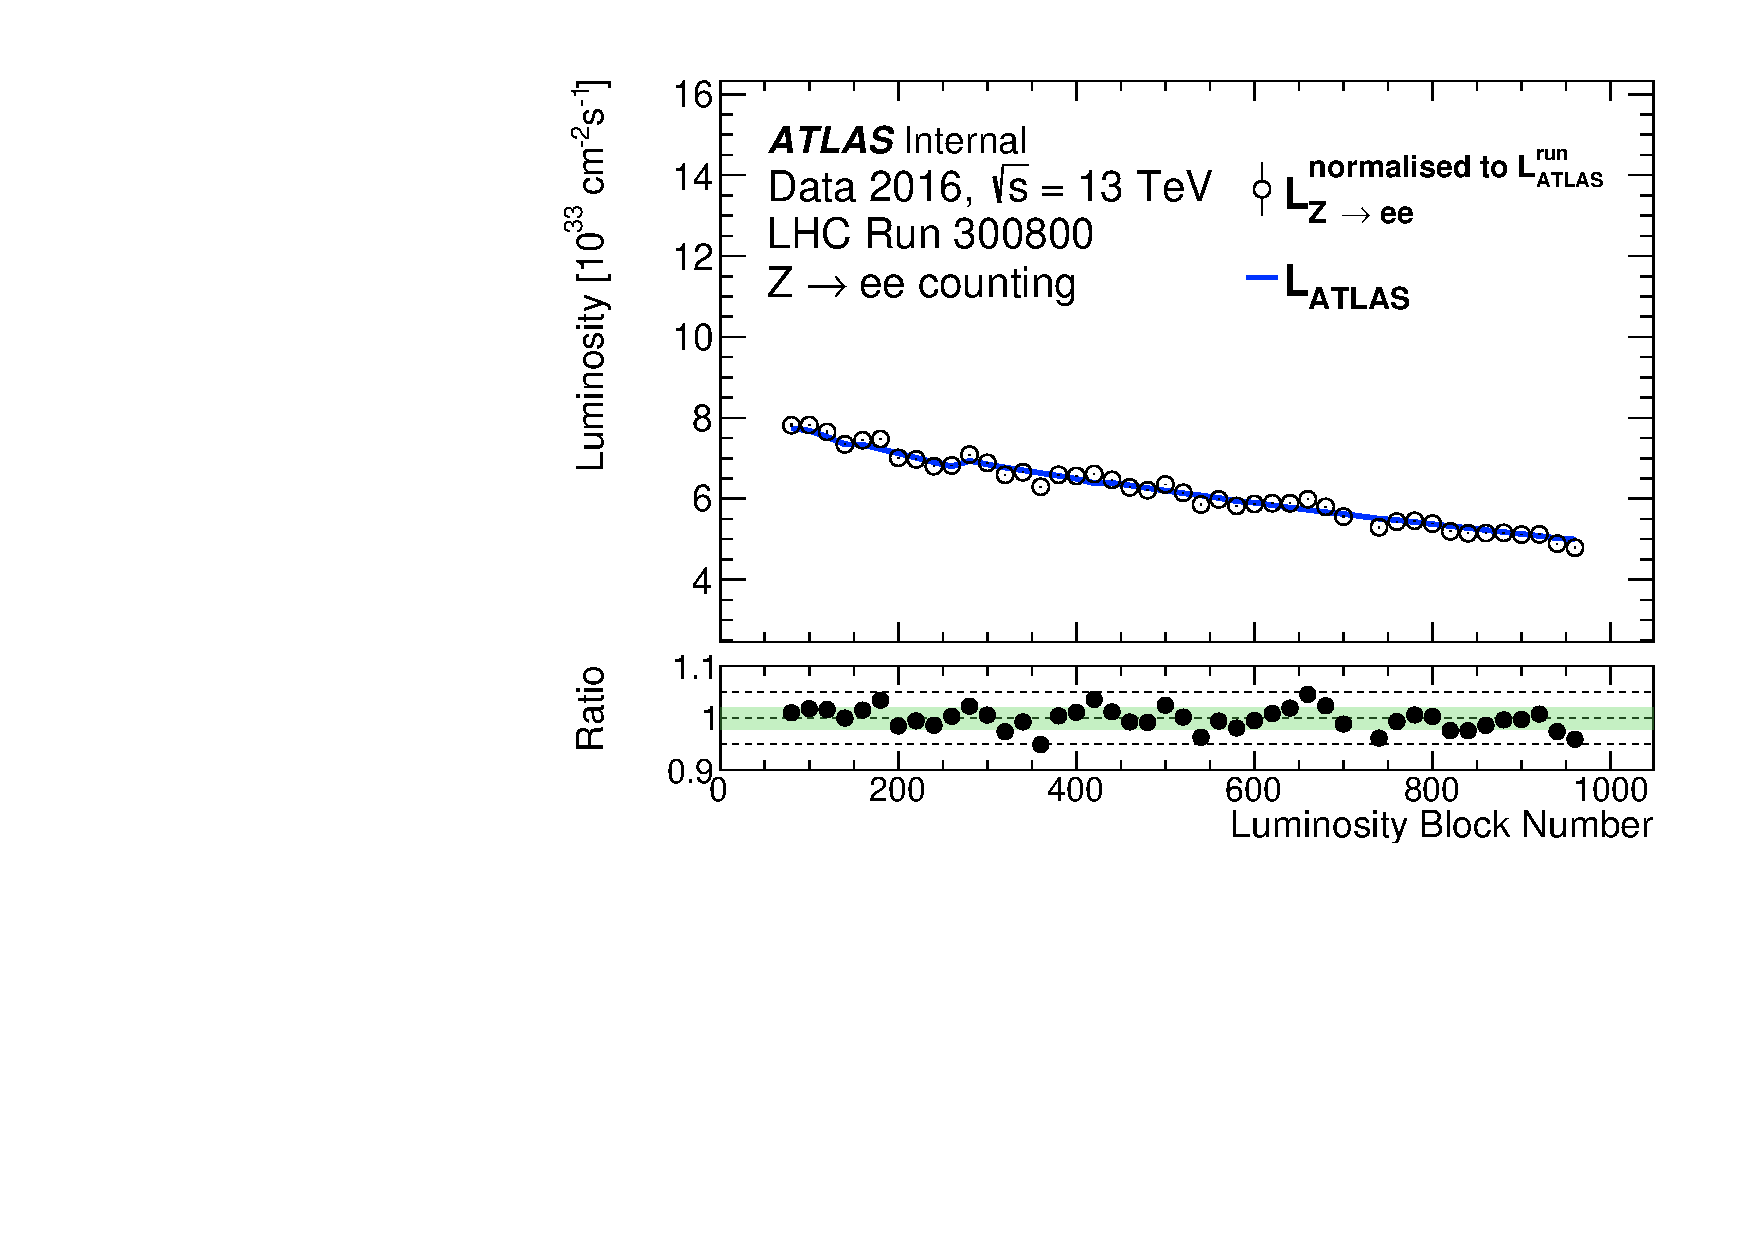
\includegraphics[width=0.48\textwidth]{figs/Zcount/Lumi/300800_Zee_vs_atlas.pdf}}\\
	\subfloat{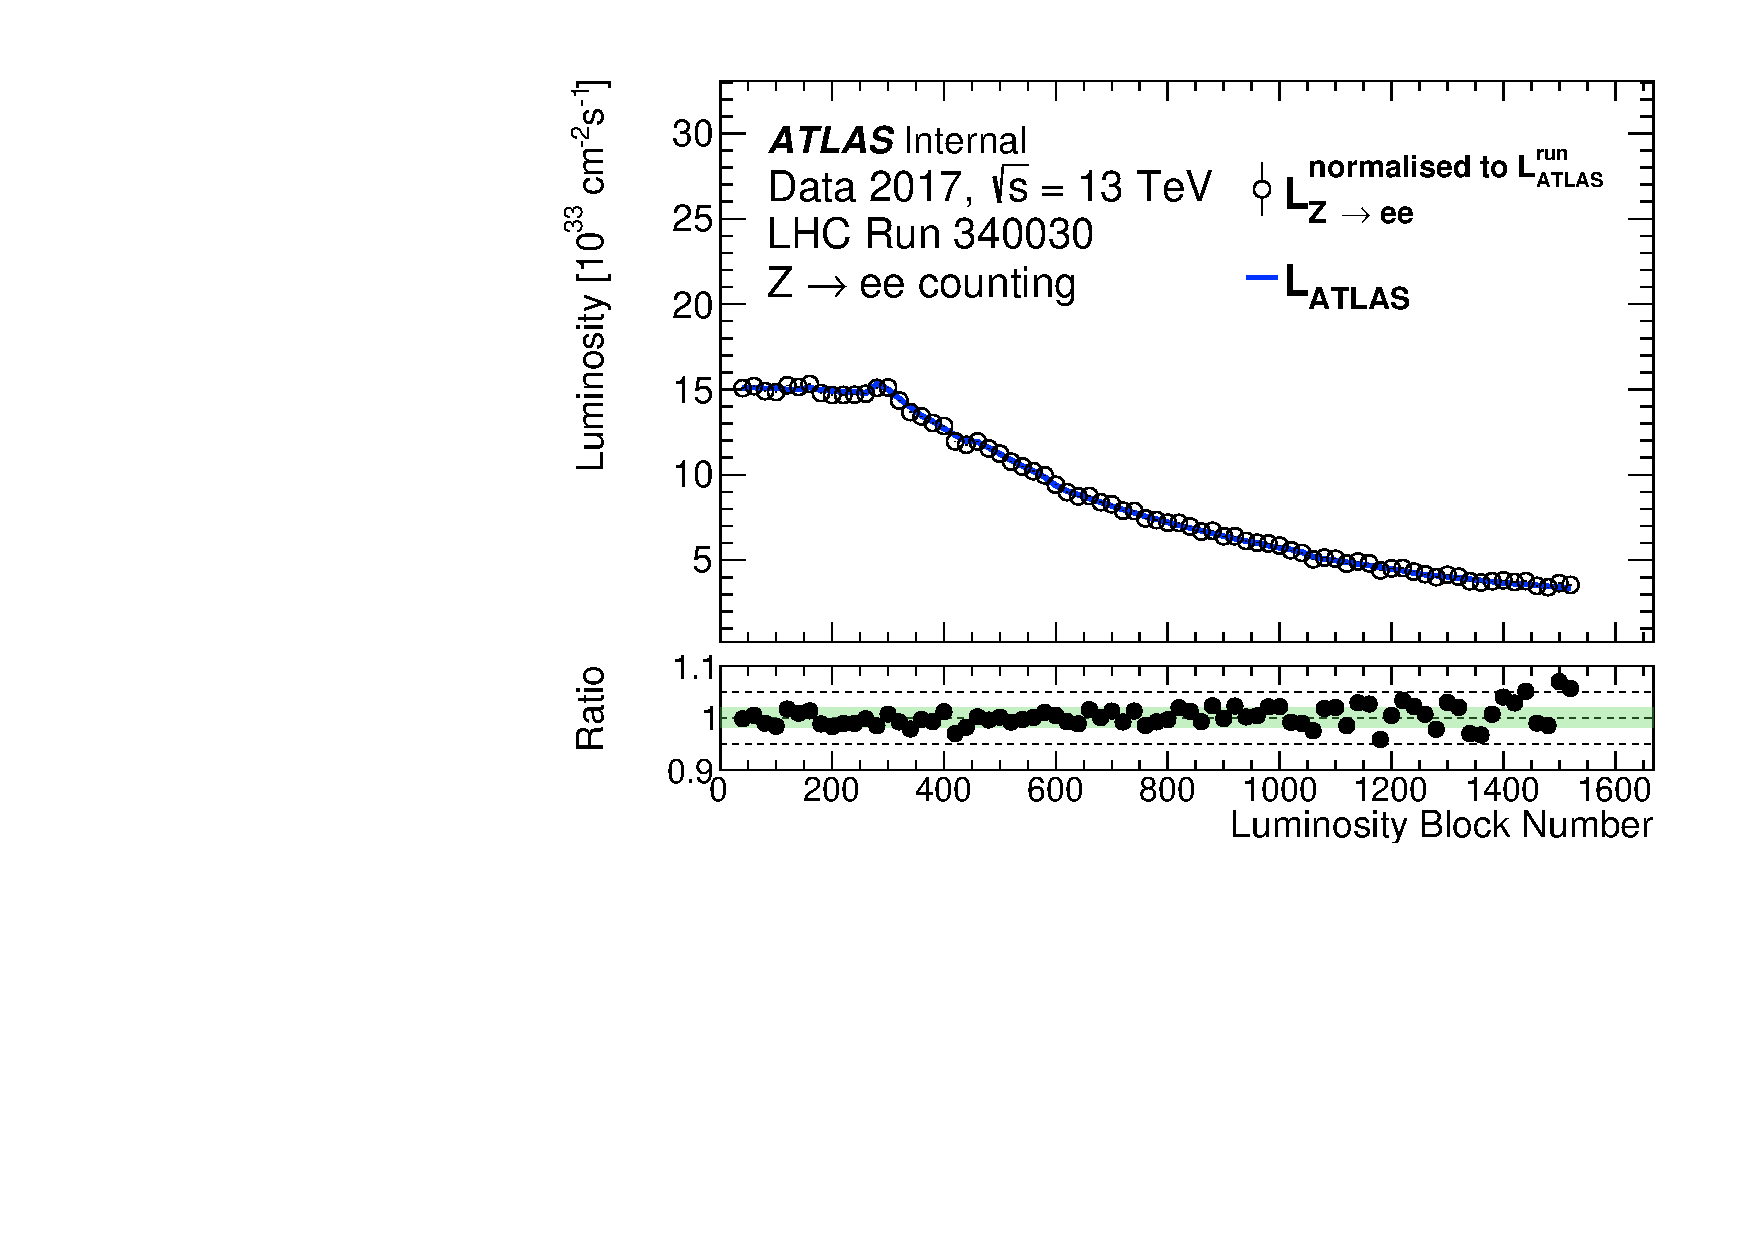
\includegraphics[width=0.48\textwidth]{figs/Zcount/Lumi/340030_Zee_vs_atlas.pdf}}
	\subfloat{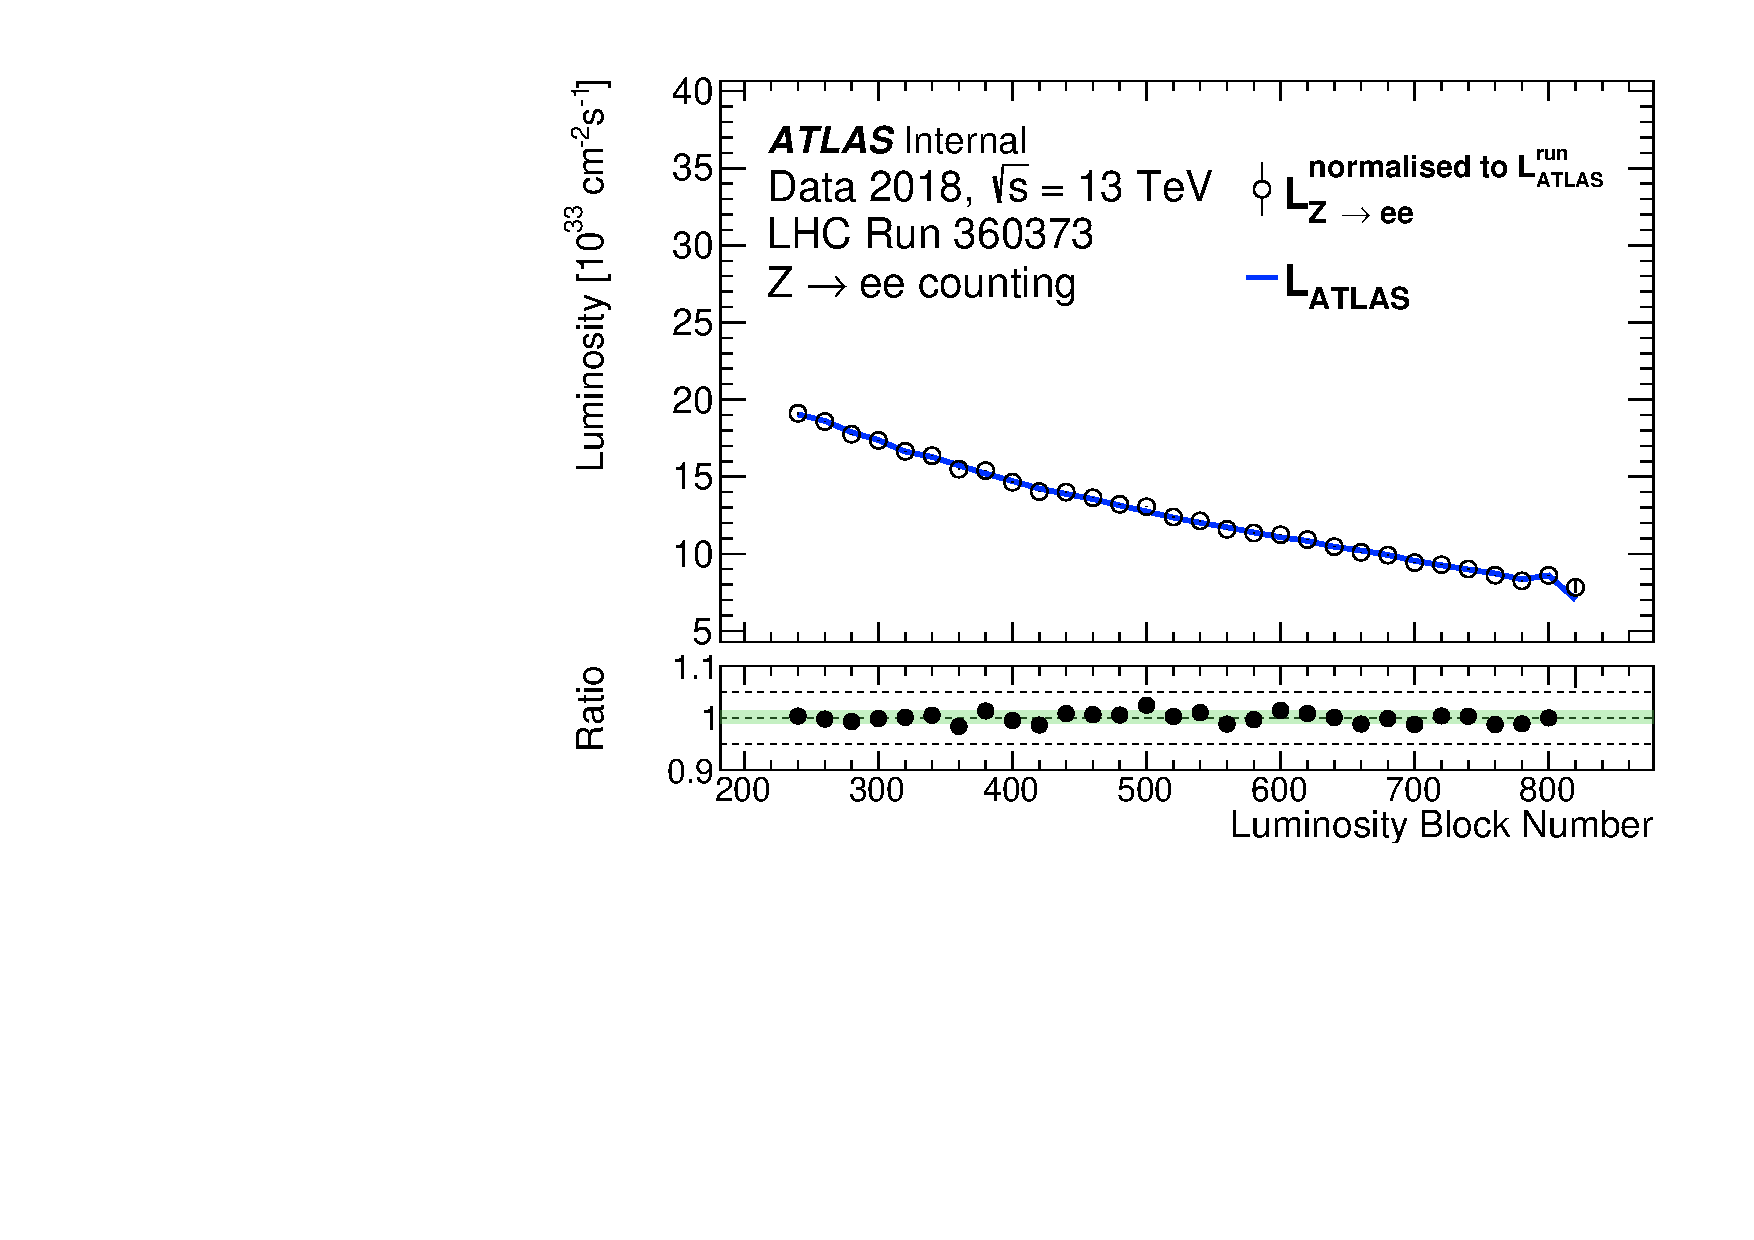
\includegraphics[width=0.48\textwidth]{figs/Zcount/Lumi/360373_Zee_vs_atlas.pdf}}
	\caption{Time-dependence of the instantaneous luminosity determined from Z-counting (open circles) and the baseline ATLAS luminosity measurement (blue lines) and their ratios (full circles), for the electron channel. The run-integrated Z-counting luminosity is normalised to the corresponding baseline ATLAS luminosity. The error bars show the statistical uncertainty of the $\mathcal{L_{Z\rightarrow \ell^+\ell^-}}$ determination. Dashed lines represent rations of 1.05, 1.0, 0.85 to guide the eye. The green band in the ratio plot contains 68\% of all points centered around the mean.}
	\label{fig:Zcount:Single run lumi electron}
\end{figure}

\subsubsection{Time-dependence of $\mathcal{L}_Z/\mathcal{L}_\text{ATLAS}$}

The ratio of the normalised $Z$-counting luminosity and the baseline ATLAS measurement~\cite{ATLAS-CONF-2019-021} can be used to study their relative stability over time for all Run-2 data-taking periods. Here the year-integrated $Z$-counting luminosity is normalised to the corresponding integrated baseline ATLAS luminosity. The run-by-run luminosity ratio is thus independent of the absolute scale of the $Z$-counting luminosity, and its spread around unity quantifies the relative stability for the two measurements. Figure~\ref{fig:Zcount:Yearly lumi electron} shows the normalised ratio of the $Z$-counting and baseline ATLAS luminosities for each data-taking period, indicating that the relative stability of the two measurements is very good.

The expected improvement in the statistical precision of the $Z$-counting method with increasing instantaneous luminosity is observed, with the spread around unity decreasing from 2015 to the following years. Furthermore, the year-to-year stability of the ATLAS luminosity scale can be monitored by normalising the $Z$-counting luminosity such that the Run-2 integrated luminosity is equal to the corresponding baseline ATLAS value. The spread of the results in Figure~\ref{fig:Zcount:Run 2 lumi electron} is approximately 0.66\%. The deviations observed within the uncorrelated year-by-year uncertainties that affect the absolute scale of the baseline ATLAS luminosity, amounting to 1.3\% for 2015/16, 1.3\% for 2017 and 1.0\% for 2018~\cite{ATLAS-CONF-2019-021}.

\begin{figure}[!htb]
	\centering
	\subfloat{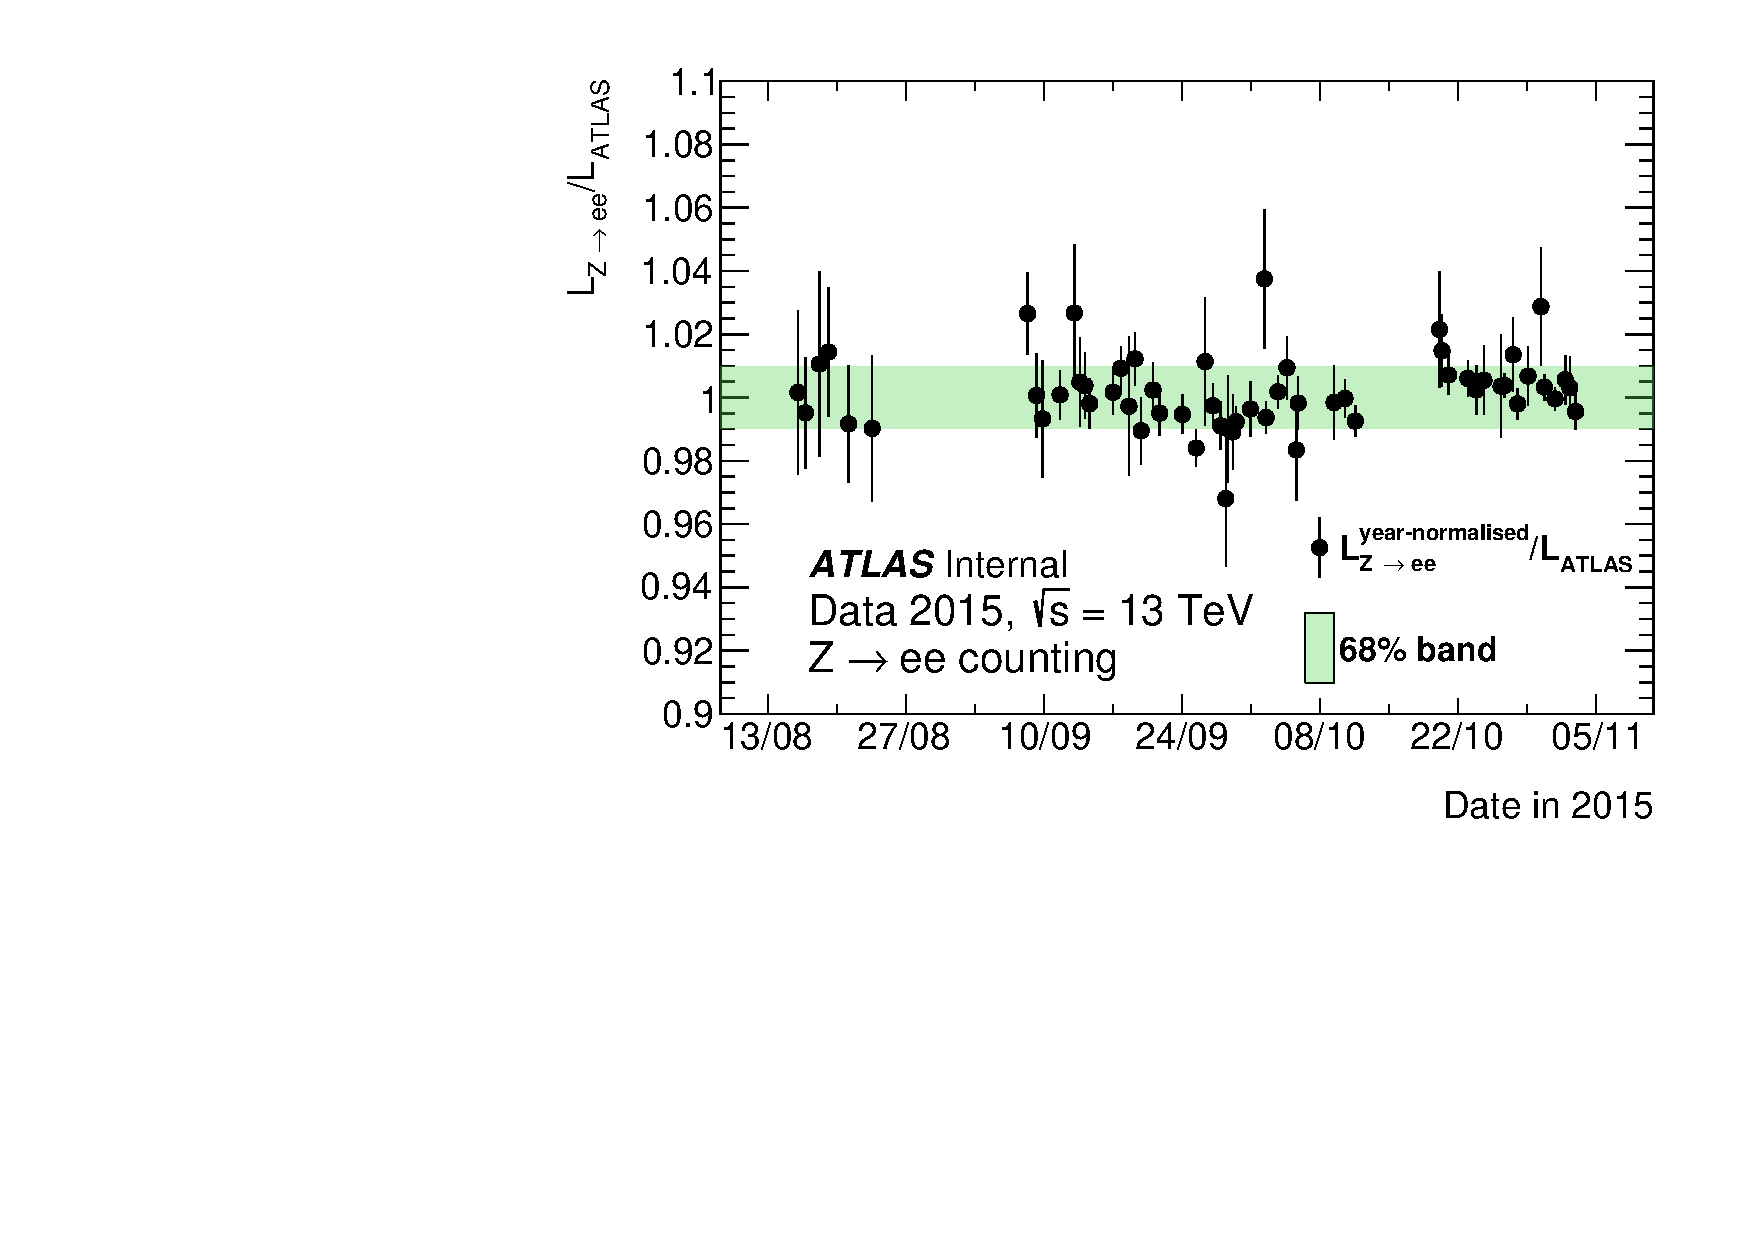
\includegraphics[width=0.48\textwidth]{figs/Zcount/Lumi/Zee_counting_data15.pdf}}
	\subfloat{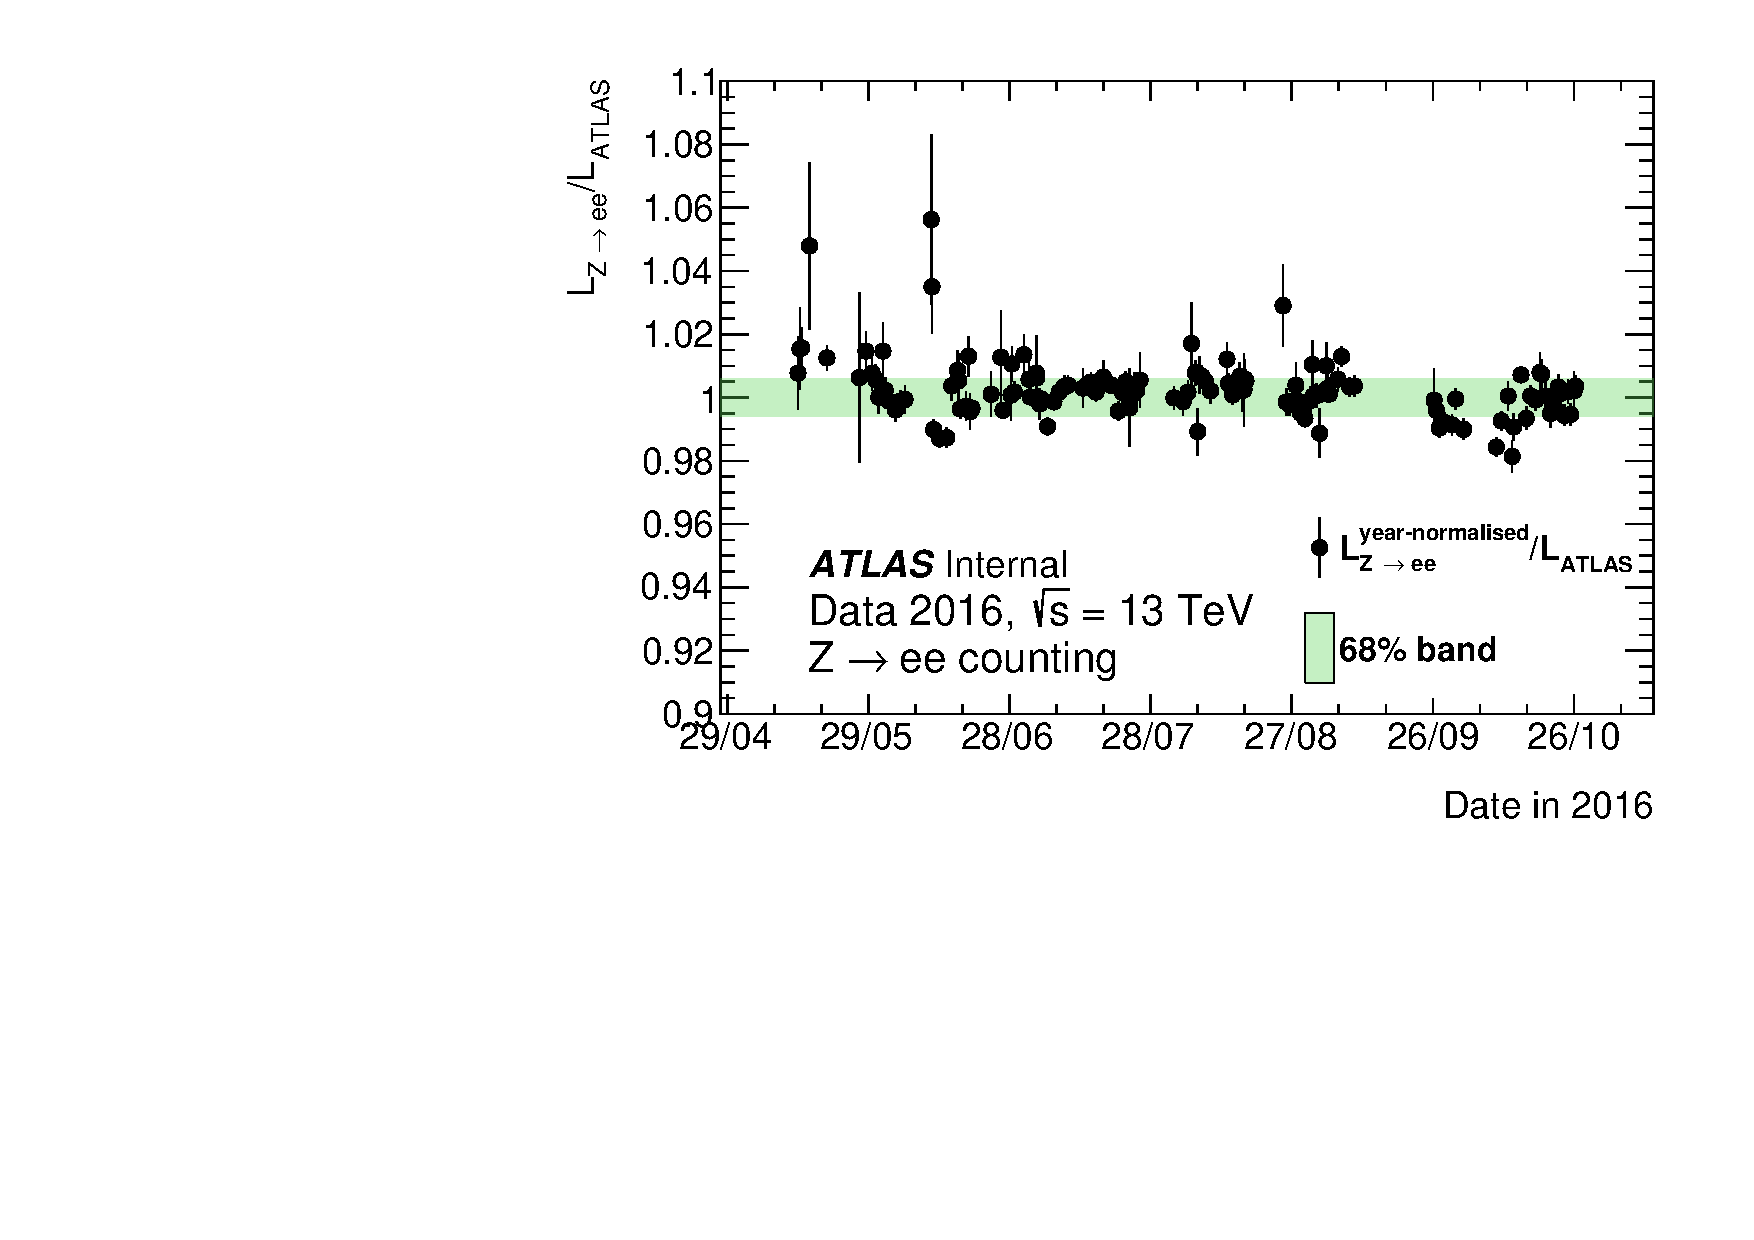
\includegraphics[width=0.48\textwidth]{figs/Zcount/Lumi/Zee_counting_data16.pdf}}\\
	\subfloat{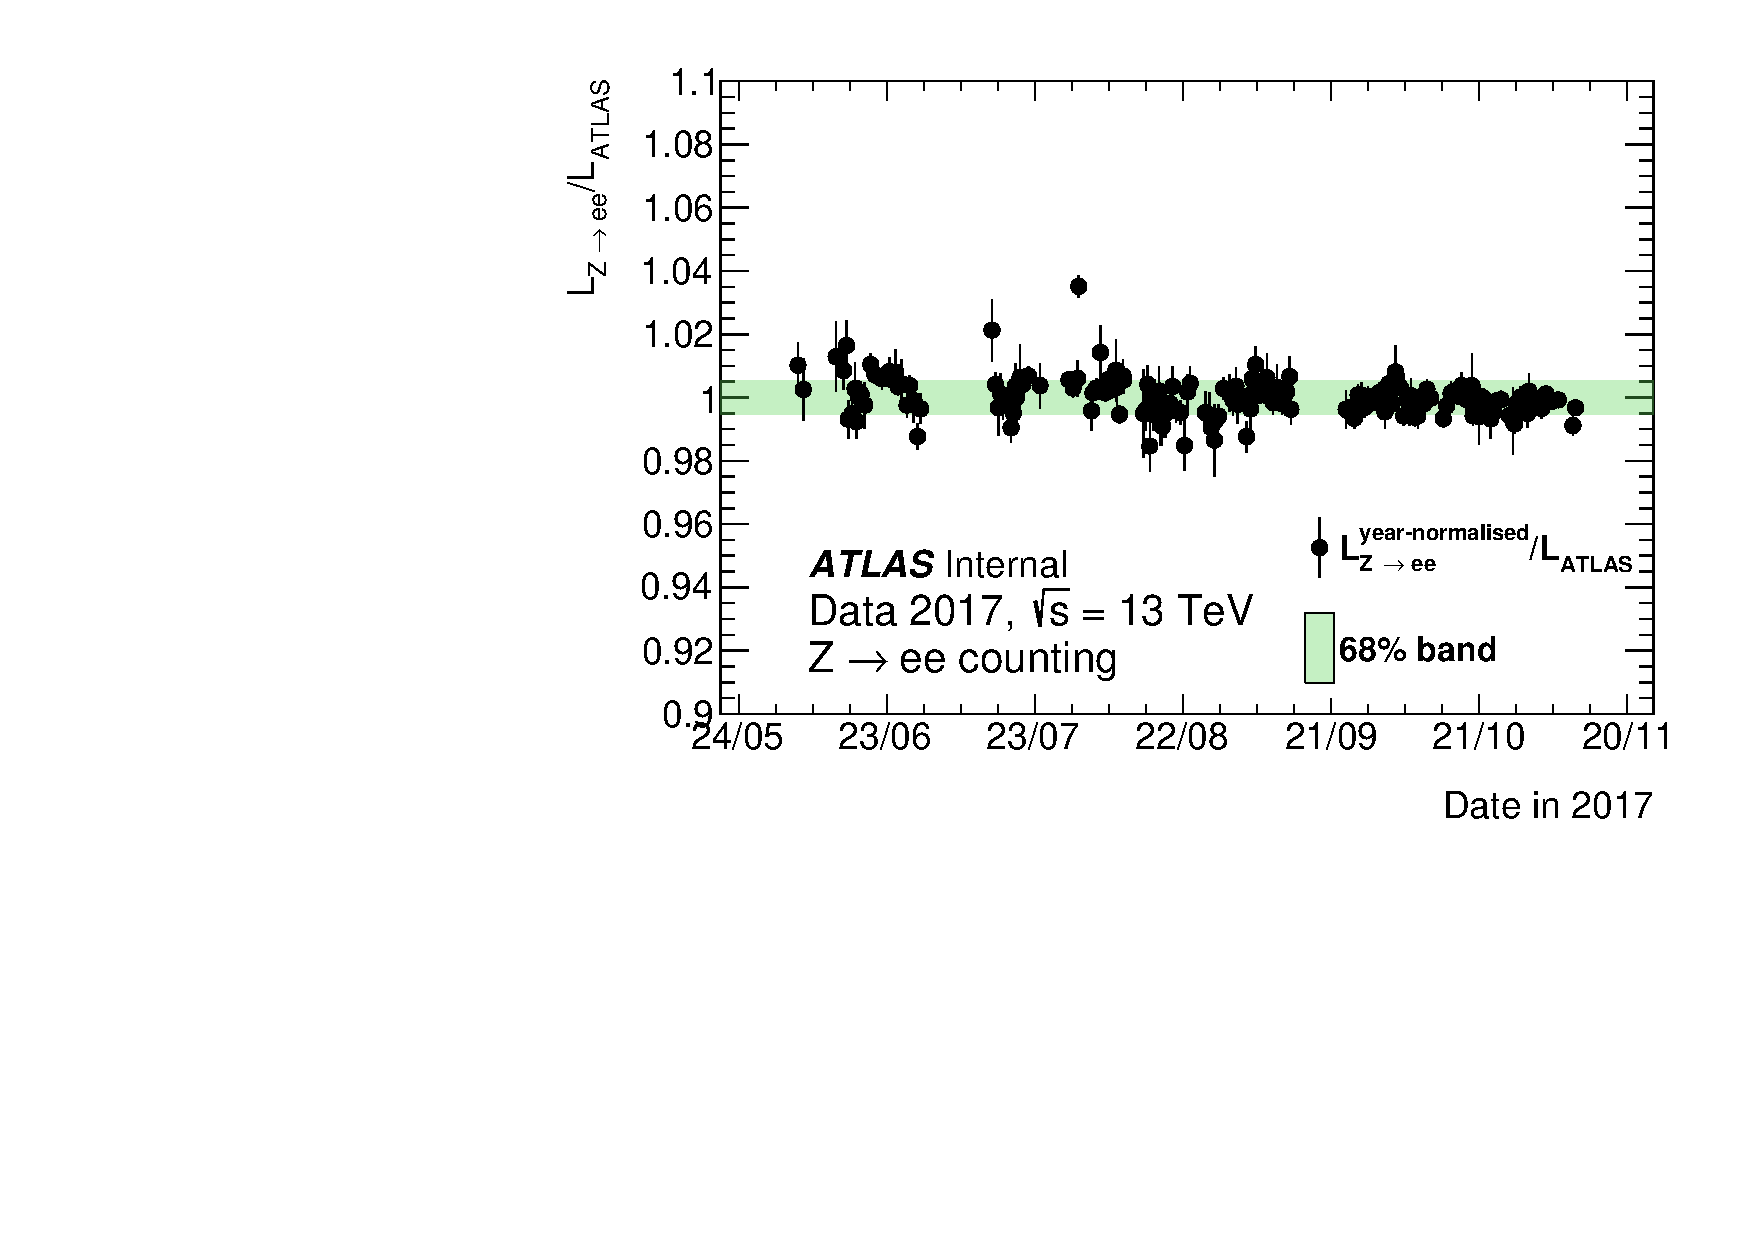
\includegraphics[width=0.48\textwidth]{figs/Zcount/Lumi/Zee_counting_data17.pdf}}
	\subfloat{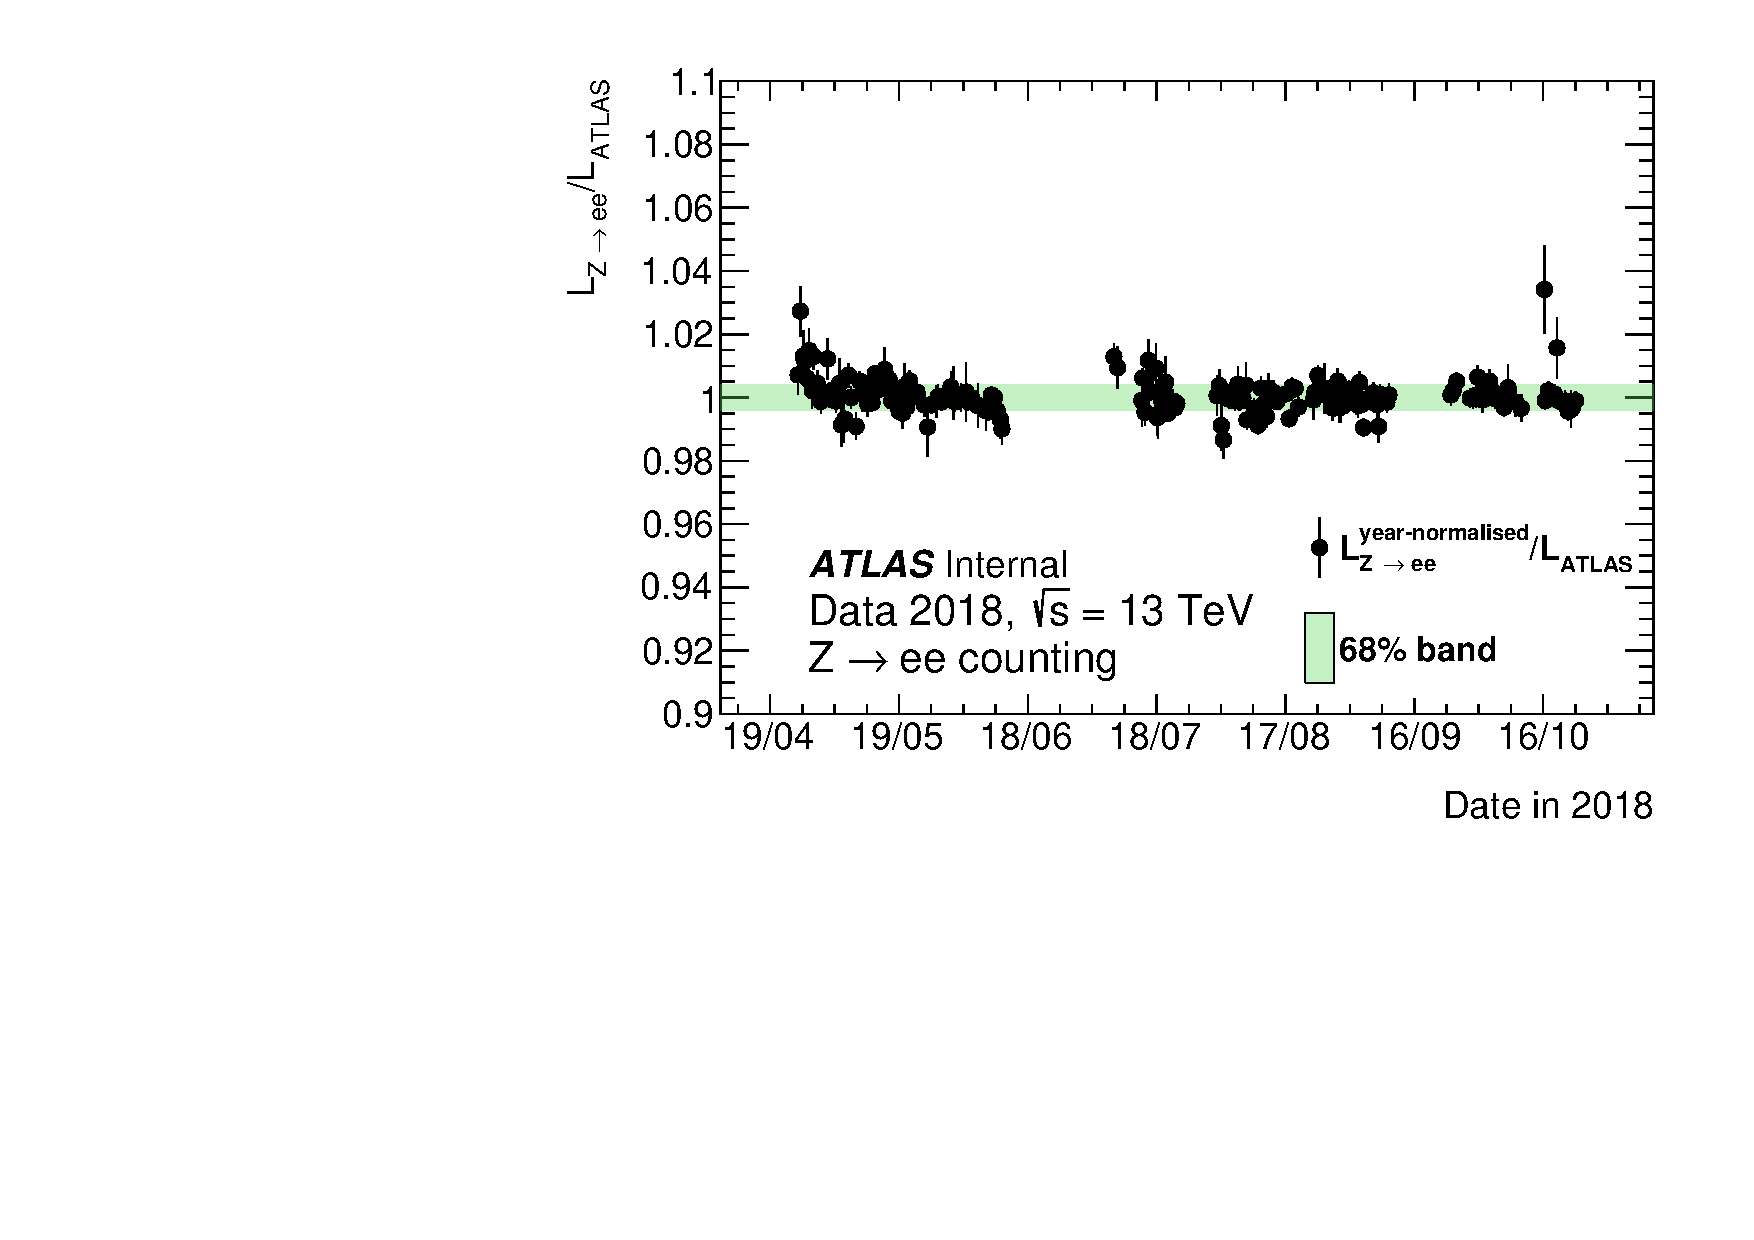
\includegraphics[width=0.48\textwidth]{figs/Zcount/Lumi/Zee_counting_data18.pdf}}
	\caption{Ratio of the integrated $Z$-counting and baseline ATLAS luminosities per LHC run taken from $pp$ collisions at $\sqrt{s}=13$~TeV for the $Z\rightarrow e^+e^-$ channel. The $Z$-counting luminosity is normalised to the integrated baseline ATLAS luminosity per data-taking period~\cite{ATLAS-CONF-2019-021}. The $x$-axis represents the date when the run started. Only ATLAS runs with a minimum length of 40 minutes are included. The error bars show statistical uncertainties only and the green bands contain 68\% of all points centered around the mean.}
	\label{fig:Zcount:Yearly lumi electron}
\end{figure}

\begin{figure}[!htb]
	\centering
	\subfloat{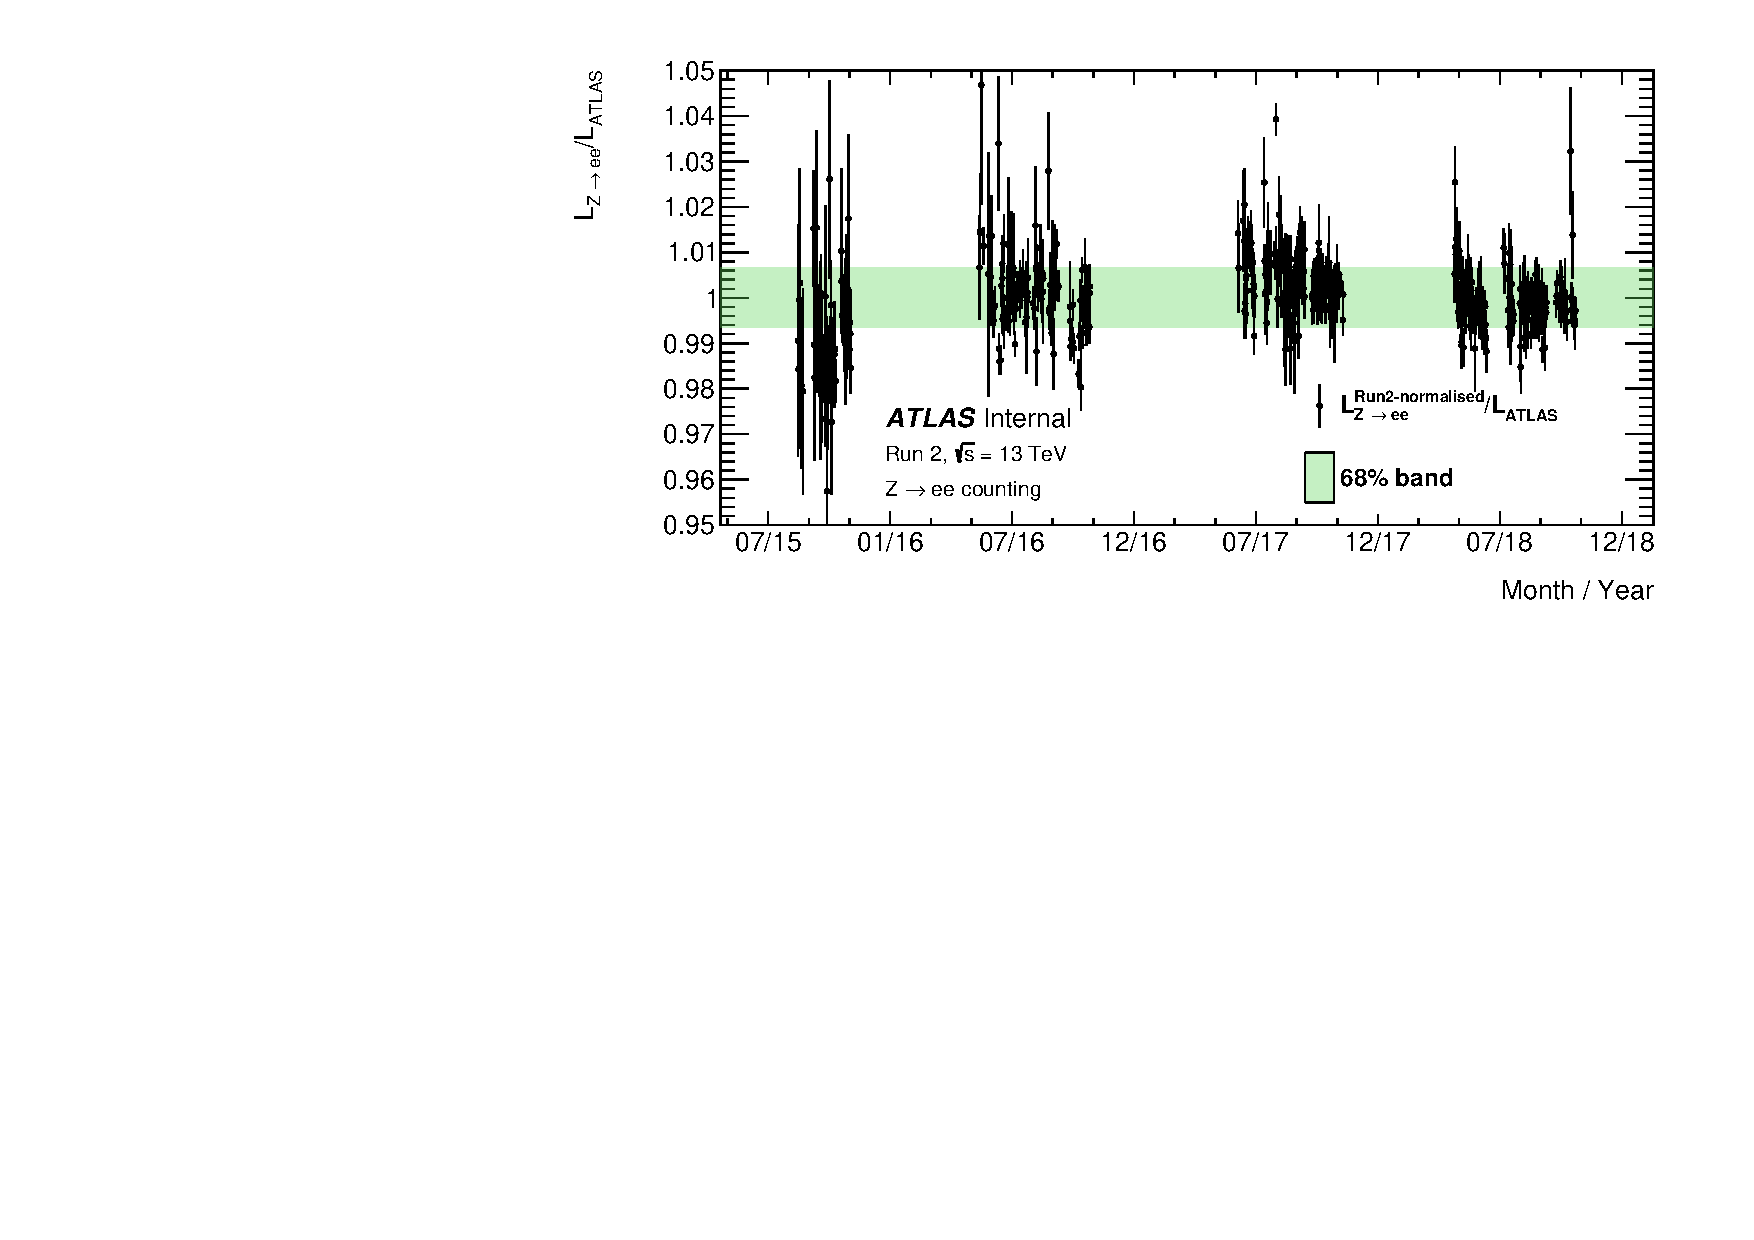
\includegraphics[width=0.98\textwidth]{figs/Zcount/Lumi/Zee_counting_data_run2.pdf}}
	\caption{Ratio of the integrated $Z$-counting and baseline ATLAS luminosities per LHC run taken from $pp$ collisions at $\sqrt{s}=13$~TeV for the $Z\rightarrow e^+e^-$ channel for the full Run-2 data taking period. The $Z$-counting luminosity is normalised to the integrated baseline ATLAS luminosity over the Run-2 data-taking period~\cite{ATLAS-CONF-2019-021}. The $x$-axis represents the date when the run started. Only ATLAS runs with a minimum length of 40 minutes are included. The error bars show statistical uncertainties only and the green bands contain 68\% of all points centered around the mean.}
	\label{fig:Zcount:Run 2 lumi electron}
\end{figure}

\clearpage

\subsection{Muon channel limitations in AnalysisBase}

The results shown throughout the previous Section were obtained adapting the Z-counting methodology to AnalysisBase, meaning the framework runs on data derivations that include some event pre-selection. In the case of the electron channel this pre-selection does not limit the results obtained, but for muon decays it means that reconstruction efficiencies will be inherently biased towards a higher efficiency. The reconstruction efficiency for muons is given by the expression shown in Equation~\ref{eq:Zcount:Single-lep reco eff} and, as shown in Table~\ref{tab:Zcount:RecoEffSelection}, probe candidates consist of inner detector tracks passing some very basic pre-selection cuts. In Tier0 data, these pre-selection cuts keep 99\% of the ID tracks, allowing for a good measurement of the reconstruction efficiency. However, in derivated data most of the pre-selection cuts apply some track removal, since the chances of ATLAS analysis requiring access to information on all tracks is very unlikely, allowing for the slimming of data files to reduce storage space usage. The tracks that are slimmed away in the derivation process tend to correspond to non-match objects, since those muon-like candidates pass the pre-selection criteria, meaning that the denominator in Equation~\ref{eq:Zcount:Single-lep reco eff} is smaller ($N^\text{OS}_\text{fail}$ is reduced), resulting in a bigger reconstruction efficiency. Table~\ref{tab:Zcount:muon reco eff} shows some numbers for all elements used in the determination of the reconstruction efficiency for different data derivations available for a given luminosity block in the 2018 data period. The table shows how the different pre-selection requirements applied in different derivations tested drastically reduce the number of tracks fulfilling the $N^\text{OS}_\text{fail}$ criteria, resulting in a difference in reconstruction efficiency of over 10\%.\\

\begin{table}[!htb]
	\centering
	\begin{tabular}{@{}cccc@{}}
		\toprule
		\multirow{2}{*}{Quantity} & \multicolumn{3}{c}{Derivation} \\ \cmidrule(l){2-4} 
		& STDM4    & MUON1    & Tier0    \\ \midrule
		$N^\text{OS}_\text{pass}$                   & 212      & 212      & 206      \\
		$N^\text{bkg}_\text{pass}$                  & 0        & 0        & 0        \\
		$N^\text{OS}_\text{fail}$                   & 21       & 42       & 57       \\
		$N^\text{bkg}_\text{fail}$                  & 6        & 13       & 14       \\ \midrule
		$\varepsilon_{\text{reco},1\mu}$ [\%]              & 93.4     & 87.9     & 82.7     \\ \bottomrule
	\end{tabular}
	\caption{Summary of the quantities that are used in the computation of the single-muon reconstruction efficiency, as shown in Equation~\ref{eq:Zcount:Single-lep reco eff} for different derivations. STDM4 is the standard derivation used in single-lepton analyses in ATLAS. MUON1 is a muon-specific derivation that lowers the selection criteria on tracks included in the data files. Tier0 refers to the numbers corresponding to the original results used in the Z-counting luminosity computation, obtained using the WZFinder tool in the DataQuality analysis framework.}
	\label{tab:Zcount:muon reco eff}
\end{table}

Moreover, the effects of the track slimming applied in the derivation process on the muon channel Z-counting is dependent on the pileup of the process. The additional proton interactions result in a higher number of low-quality tracks that, although originally accounted for in the standard Z-counting methodology, are removed from the stored data in usual ATLAS derivations. This results in a time-dependent effect observed in muon channel Z-counting performed on AnalysisBase, since 2017 and 2018 data was taken with a higher pileup than the previous Run 2 years, resulting in a change in efficiency behaviour that biases the luminosity obtained with the Z-counting methodology, as one can observe in Figure~\ref{fig:Zcount:Run 2 lumi muon}. It can be inferred in the Figure that late-Run 2 data results into a Z-counting luminosity dip, stemming from a bigger effect of ID track slimming in the derivation process, increasing the reconstruction efficiency measurement and therefore decreasing the luminosity estimation (see Equation~\ref{eq:Zcount:ZLumi_app}). The effect can also be inferred in Figure~\ref{fig:Zcount:Run 2 lumi channel comp}, where the dip in the luminosity obtained in the muon channel results into an increase with respect to that measured in the electron channel in late Run 2 runs, where higher pileup values where recorded and the effects of track slimming are more severe in the luminosity determination in the muon channel.\\

Considering the limitations the AnalysisBase framework presents in the muon channel, the results presented in the analysis will be based on the original Z-counting methodology developed in the DataQuality framework, updated to the latest luminosity Tag11 official ATLAS measurement.

\begin{figure}[!htb]
	\centering
	\subfloat{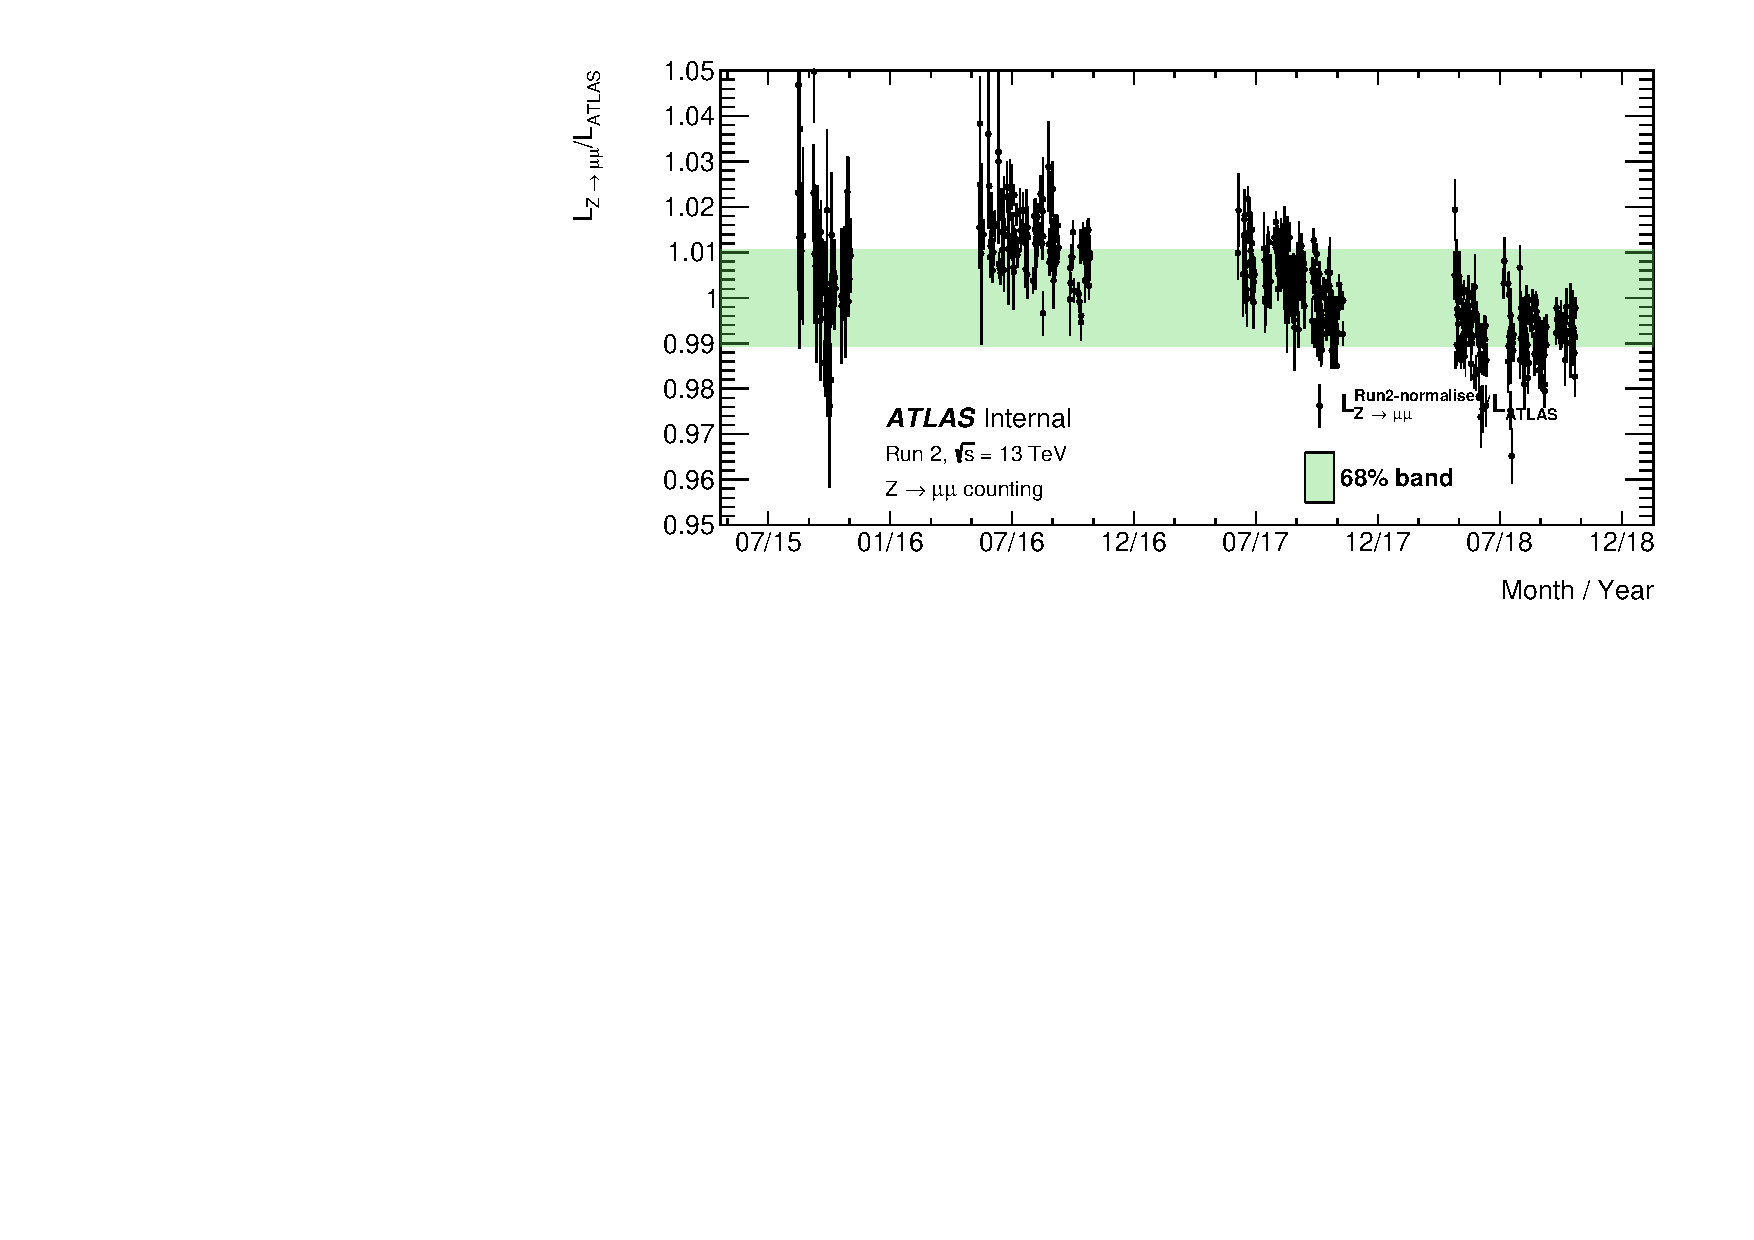
\includegraphics[width=0.98\textwidth]{figs/Zcount/Lumi/Zmumu_counting_data_run2.pdf}}
	\caption{Ratio of the integrated $Z$-counting and baseline ATLAS luminosities per LHC run taken from $pp$ collisions at $\sqrt{s}=13$~TeV for the $Z\rightarrow \mu^+\mu^-$ channel for the full Run-2 data taking period. The $Z$-counting luminosity is normalised to the integrated baseline ATLAS luminosity over the Run-2 data-taking period~\cite{ATLAS-CONF-2019-021}. The $x$-axis represents the date when the run started. Only ATLAS runs with a minimum length of 40 minutes are included. The error bars show statistical uncertainties only and the green bands contain 68\% of all points centered around the mean.}
	\label{fig:Zcount:Run 2 lumi muon}
\end{figure}

\begin{figure}[!htb]
	\centering
	\subfloat{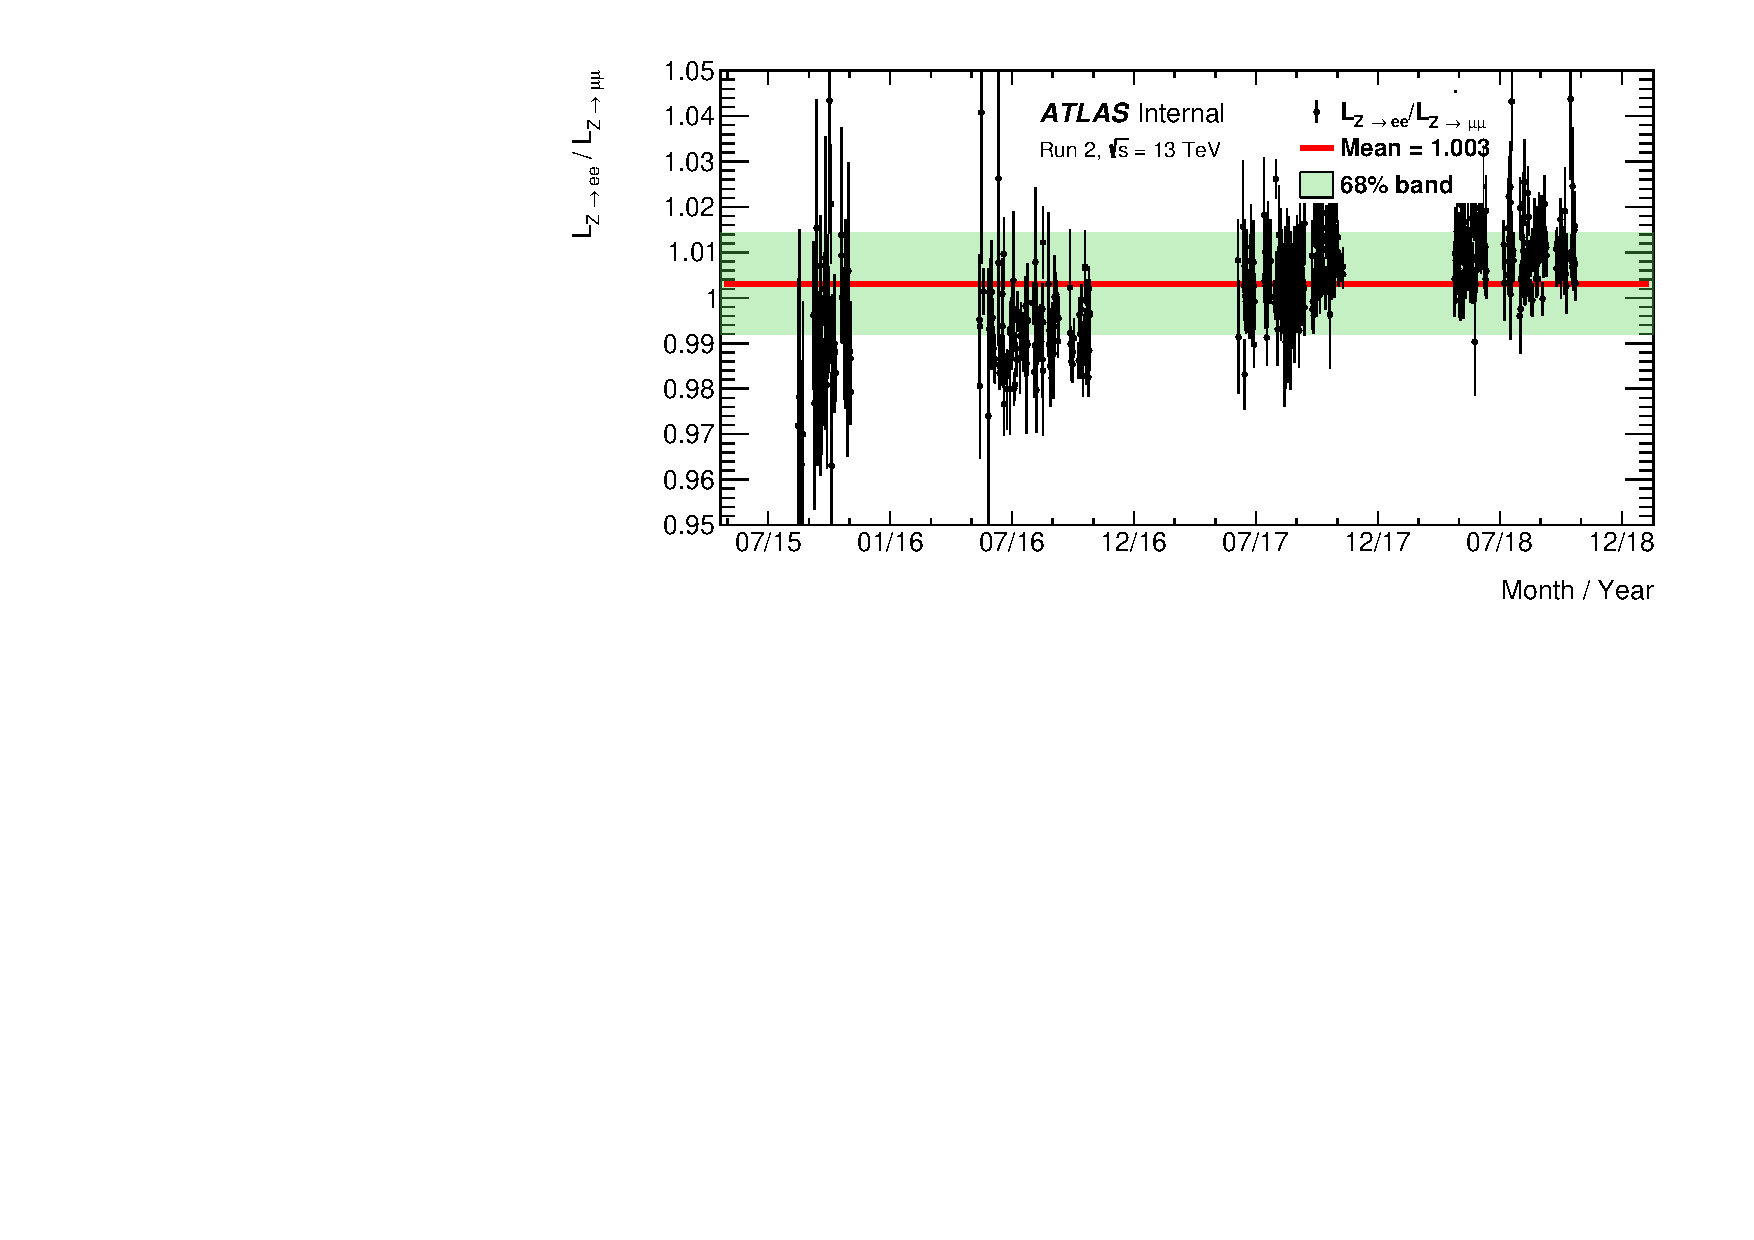
\includegraphics[width=0.98\textwidth]{figs/Zcount/Lumi/channel_comp_data_run2.pdf}}
	\caption{Ratio of the integrated $Z$-counting $Z\rightarrow e^+e^-$ and $Z\rightarrow \mu^+\mu^-$ luminosities per LHC run taken from $pp$ collisions at $\sqrt{s}=13$~TeV for the full Run-2 data taking period. The red line indicated the mean of the distribution obtained from a fit to a constant. The error bars show statistical uncertainties only and the green bands contain 68\% of all points centered around the mean.}
	\label{fig:Zcount:Run 2 lumi channel comp}
\end{figure}
